\documentclass[11pt]{article}

    \usepackage[breakable]{tcolorbox}
    \usepackage{parskip} % Stop auto-indenting (to mimic markdown behaviour)
    
    \usepackage{iftex}
    \ifPDFTeX
    	\usepackage[T1]{fontenc}
    	\usepackage{mathpazo}
    \else
    	\usepackage{fontspec}
    \fi
	\usepackage[UTF8]{ctex}
    % Basic figure setup, for now with no caption control since it's done
    % automatically by Pandoc (which extracts ![](path) syntax from Markdown).
    \usepackage{graphicx}
    % Maintain compatibility with old templates. Remove in nbconvert 6.0
    \let\Oldincludegraphics\includegraphics
    % Ensure that by default, figures have no caption (until we provide a
    % proper Figure object with a Caption API and a way to capture that
    % in the conversion process - todo).
    \usepackage{caption}
    \DeclareCaptionFormat{nocaption}{}
    \captionsetup{format=nocaption,aboveskip=0pt,belowskip=0pt}

    \usepackage[Export]{adjustbox} % Used to constrain images to a maximum size
    \adjustboxset{max size={0.9\linewidth}{0.9\paperheight}}
    \usepackage{float}
    \floatplacement{figure}{H} % forces figures to be placed at the correct location
    \usepackage{xcolor} % Allow colors to be defined
    \usepackage{enumerate} % Needed for markdown enumerations to work
    \usepackage{geometry} % Used to adjust the document margins
    \usepackage{amsmath} % Equations
    \usepackage{amssymb} % Equations
    \usepackage{textcomp} % defines textquotesingle
    % Hack from http://tex.stackexchange.com/a/47451/13684:
    \AtBeginDocument{%
        \def\PYZsq{\textquotesingle}% Upright quotes in Pygmentized code
    }
    \usepackage{upquote} % Upright quotes for verbatim code
    \usepackage{eurosym} % defines \euro
    \usepackage[mathletters]{ucs} % Extended unicode (utf-8) support
    \usepackage{fancyvrb} % verbatim replacement that allows latex
    \usepackage{grffile} % extends the file name processing of package graphics 
                         % to support a larger range
    \makeatletter % fix for grffile with XeLaTeX
    \def\Gread@@xetex#1{%
      \IfFileExists{"\Gin@base".bb}%
      {\Gread@eps{\Gin@base.bb}}%
      {\Gread@@xetex@aux#1}%
    }
    \makeatother

    % The hyperref package gives us a pdf with properly built
    % internal navigation ('pdf bookmarks' for the table of contents,
    % internal cross-reference links, web links for URLs, etc.)
    \usepackage{hyperref}
    % The default LaTeX title has an obnoxious amount of whitespace. By default,
    % titling removes some of it. It also provides customization options.
    \usepackage{titling}
    \usepackage{longtable} % longtable support required by pandoc >1.10
    \usepackage{booktabs}  % table support for pandoc > 1.12.2
    \usepackage[inline]{enumitem} % IRkernel/repr support (it uses the enumerate* environment)
   % \usepackage[normalem]{ulem} % ulem is needed to support strikethroughs (\sout)
                                % normalem makes italics be italics, not underlines
    \usepackage{mathrsfs}
    

    
    % Colors for the hyperref package
    \definecolor{urlcolor}{rgb}{0,.145,.698}
    \definecolor{linkcolor}{rgb}{.71,0.21,0.01}
    \definecolor{citecolor}{rgb}{.12,.54,.11}

    % ANSI colors
    \definecolor{ansi-black}{HTML}{3E424D}
    \definecolor{ansi-black-intense}{HTML}{282C36}
    \definecolor{ansi-red}{HTML}{E75C58}
    \definecolor{ansi-red-intense}{HTML}{B22B31}
    \definecolor{ansi-green}{HTML}{00A250}
    \definecolor{ansi-green-intense}{HTML}{007427}
    \definecolor{ansi-yellow}{HTML}{DDB62B}
    \definecolor{ansi-yellow-intense}{HTML}{B27D12}
    \definecolor{ansi-blue}{HTML}{208FFB}
    \definecolor{ansi-blue-intense}{HTML}{0065CA}
    \definecolor{ansi-magenta}{HTML}{D160C4}
    \definecolor{ansi-magenta-intense}{HTML}{A03196}
    \definecolor{ansi-cyan}{HTML}{60C6C8}
    \definecolor{ansi-cyan-intense}{HTML}{258F8F}
    \definecolor{ansi-white}{HTML}{C5C1B4}
    \definecolor{ansi-white-intense}{HTML}{A1A6B2}
    \definecolor{ansi-default-inverse-fg}{HTML}{FFFFFF}
    \definecolor{ansi-default-inverse-bg}{HTML}{000000}

    % commands and environments needed by pandoc snippets
    % extracted from the output of `pandoc -s`
    \providecommand{\tightlist}{%
      \setlength{\itemsep}{0pt}\setlength{\parskip}{0pt}}
    \DefineVerbatimEnvironment{Highlighting}{Verbatim}{commandchars=\\\{\}}
    % Add ',fontsize=\small' for more characters per line
    \newenvironment{Shaded}{}{}
    \newcommand{\KeywordTok}[1]{\textcolor[rgb]{0.00,0.44,0.13}{\textbf{{#1}}}}
    \newcommand{\DataTypeTok}[1]{\textcolor[rgb]{0.56,0.13,0.00}{{#1}}}
    \newcommand{\DecValTok}[1]{\textcolor[rgb]{0.25,0.63,0.44}{{#1}}}
    \newcommand{\BaseNTok}[1]{\textcolor[rgb]{0.25,0.63,0.44}{{#1}}}
    \newcommand{\FloatTok}[1]{\textcolor[rgb]{0.25,0.63,0.44}{{#1}}}
    \newcommand{\CharTok}[1]{\textcolor[rgb]{0.25,0.44,0.63}{{#1}}}
    \newcommand{\StringTok}[1]{\textcolor[rgb]{0.25,0.44,0.63}{{#1}}}
    \newcommand{\CommentTok}[1]{\textcolor[rgb]{0.38,0.63,0.69}{\textit{{#1}}}}
    \newcommand{\OtherTok}[1]{\textcolor[rgb]{0.00,0.44,0.13}{{#1}}}
    \newcommand{\AlertTok}[1]{\textcolor[rgb]{1.00,0.00,0.00}{\textbf{{#1}}}}
    \newcommand{\FunctionTok}[1]{\textcolor[rgb]{0.02,0.16,0.49}{{#1}}}
    \newcommand{\RegionMarkerTok}[1]{{#1}}
    \newcommand{\ErrorTok}[1]{\textcolor[rgb]{1.00,0.00,0.00}{\textbf{{#1}}}}
    \newcommand{\NormalTok}[1]{{#1}}
    
    % Additional commands for more recent versions of Pandoc
    \newcommand{\ConstantTok}[1]{\textcolor[rgb]{0.53,0.00,0.00}{{#1}}}
    \newcommand{\SpecialCharTok}[1]{\textcolor[rgb]{0.25,0.44,0.63}{{#1}}}
    \newcommand{\VerbatimStringTok}[1]{\textcolor[rgb]{0.25,0.44,0.63}{{#1}}}
    \newcommand{\SpecialStringTok}[1]{\textcolor[rgb]{0.73,0.40,0.53}{{#1}}}
    \newcommand{\ImportTok}[1]{{#1}}
    \newcommand{\DocumentationTok}[1]{\textcolor[rgb]{0.73,0.13,0.13}{\textit{{#1}}}}
    \newcommand{\AnnotationTok}[1]{\textcolor[rgb]{0.38,0.63,0.69}{\textbf{\textit{{#1}}}}}
    \newcommand{\CommentVarTok}[1]{\textcolor[rgb]{0.38,0.63,0.69}{\textbf{\textit{{#1}}}}}
    \newcommand{\VariableTok}[1]{\textcolor[rgb]{0.10,0.09,0.49}{{#1}}}
    \newcommand{\ControlFlowTok}[1]{\textcolor[rgb]{0.00,0.44,0.13}{\textbf{{#1}}}}
    \newcommand{\OperatorTok}[1]{\textcolor[rgb]{0.40,0.40,0.40}{{#1}}}
    \newcommand{\BuiltInTok}[1]{{#1}}
    \newcommand{\ExtensionTok}[1]{{#1}}
    \newcommand{\PreprocessorTok}[1]{\textcolor[rgb]{0.74,0.48,0.00}{{#1}}}
    \newcommand{\AttributeTok}[1]{\textcolor[rgb]{0.49,0.56,0.16}{{#1}}}
    \newcommand{\InformationTok}[1]{\textcolor[rgb]{0.38,0.63,0.69}{\textbf{\textit{{#1}}}}}
    \newcommand{\WarningTok}[1]{\textcolor[rgb]{0.38,0.63,0.69}{\textbf{\textit{{#1}}}}}
    
    
    % Define a nice break command that doesn't care if a line doesn't already
    % exist.
    \def\br{\hspace*{\fill} \\* }
    % Math Jax compatibility definitions
    \def\gt{>}
    \def\lt{<}
    \let\Oldtex\TeX
    \let\Oldlatex\LaTeX
    \renewcommand{\TeX}{\textrm{\Oldtex}}
    \renewcommand{\LaTeX}{\textrm{\Oldlatex}}
    % Document parameters
    % Document title
    \title{作业清单(5/11)}
    \author{唐麒}
    
    
    
    
    
% Pygments definitions
\makeatletter
\def\PY@reset{\let\PY@it=\relax \let\PY@bf=\relax%
    \let\PY@ul=\relax \let\PY@tc=\relax%
    \let\PY@bc=\relax \let\PY@ff=\relax}
\def\PY@tok#1{\csname PY@tok@#1\endcsname}
\def\PY@toks#1+{\ifx\relax#1\empty\else%
    \PY@tok{#1}\expandafter\PY@toks\fi}
\def\PY@do#1{\PY@bc{\PY@tc{\PY@ul{%
    \PY@it{\PY@bf{\PY@ff{#1}}}}}}}
\def\PY#1#2{\PY@reset\PY@toks#1+\relax+\PY@do{#2}}

\expandafter\def\csname PY@tok@w\endcsname{\def\PY@tc##1{\textcolor[rgb]{0.73,0.73,0.73}{##1}}}
\expandafter\def\csname PY@tok@c\endcsname{\let\PY@it=\textit\def\PY@tc##1{\textcolor[rgb]{0.25,0.50,0.50}{##1}}}
\expandafter\def\csname PY@tok@cp\endcsname{\def\PY@tc##1{\textcolor[rgb]{0.74,0.48,0.00}{##1}}}
\expandafter\def\csname PY@tok@k\endcsname{\let\PY@bf=\textbf\def\PY@tc##1{\textcolor[rgb]{0.00,0.50,0.00}{##1}}}
\expandafter\def\csname PY@tok@kp\endcsname{\def\PY@tc##1{\textcolor[rgb]{0.00,0.50,0.00}{##1}}}
\expandafter\def\csname PY@tok@kt\endcsname{\def\PY@tc##1{\textcolor[rgb]{0.69,0.00,0.25}{##1}}}
\expandafter\def\csname PY@tok@o\endcsname{\def\PY@tc##1{\textcolor[rgb]{0.40,0.40,0.40}{##1}}}
\expandafter\def\csname PY@tok@ow\endcsname{\let\PY@bf=\textbf\def\PY@tc##1{\textcolor[rgb]{0.67,0.13,1.00}{##1}}}
\expandafter\def\csname PY@tok@nb\endcsname{\def\PY@tc##1{\textcolor[rgb]{0.00,0.50,0.00}{##1}}}
\expandafter\def\csname PY@tok@nf\endcsname{\def\PY@tc##1{\textcolor[rgb]{0.00,0.00,1.00}{##1}}}
\expandafter\def\csname PY@tok@nc\endcsname{\let\PY@bf=\textbf\def\PY@tc##1{\textcolor[rgb]{0.00,0.00,1.00}{##1}}}
\expandafter\def\csname PY@tok@nn\endcsname{\let\PY@bf=\textbf\def\PY@tc##1{\textcolor[rgb]{0.00,0.00,1.00}{##1}}}
\expandafter\def\csname PY@tok@ne\endcsname{\let\PY@bf=\textbf\def\PY@tc##1{\textcolor[rgb]{0.82,0.25,0.23}{##1}}}
\expandafter\def\csname PY@tok@nv\endcsname{\def\PY@tc##1{\textcolor[rgb]{0.10,0.09,0.49}{##1}}}
\expandafter\def\csname PY@tok@no\endcsname{\def\PY@tc##1{\textcolor[rgb]{0.53,0.00,0.00}{##1}}}
\expandafter\def\csname PY@tok@nl\endcsname{\def\PY@tc##1{\textcolor[rgb]{0.63,0.63,0.00}{##1}}}
\expandafter\def\csname PY@tok@ni\endcsname{\let\PY@bf=\textbf\def\PY@tc##1{\textcolor[rgb]{0.60,0.60,0.60}{##1}}}
\expandafter\def\csname PY@tok@na\endcsname{\def\PY@tc##1{\textcolor[rgb]{0.49,0.56,0.16}{##1}}}
\expandafter\def\csname PY@tok@nt\endcsname{\let\PY@bf=\textbf\def\PY@tc##1{\textcolor[rgb]{0.00,0.50,0.00}{##1}}}
\expandafter\def\csname PY@tok@nd\endcsname{\def\PY@tc##1{\textcolor[rgb]{0.67,0.13,1.00}{##1}}}
\expandafter\def\csname PY@tok@s\endcsname{\def\PY@tc##1{\textcolor[rgb]{0.73,0.13,0.13}{##1}}}
\expandafter\def\csname PY@tok@sd\endcsname{\let\PY@it=\textit\def\PY@tc##1{\textcolor[rgb]{0.73,0.13,0.13}{##1}}}
\expandafter\def\csname PY@tok@si\endcsname{\let\PY@bf=\textbf\def\PY@tc##1{\textcolor[rgb]{0.73,0.40,0.53}{##1}}}
\expandafter\def\csname PY@tok@se\endcsname{\let\PY@bf=\textbf\def\PY@tc##1{\textcolor[rgb]{0.73,0.40,0.13}{##1}}}
\expandafter\def\csname PY@tok@sr\endcsname{\def\PY@tc##1{\textcolor[rgb]{0.73,0.40,0.53}{##1}}}
\expandafter\def\csname PY@tok@ss\endcsname{\def\PY@tc##1{\textcolor[rgb]{0.10,0.09,0.49}{##1}}}
\expandafter\def\csname PY@tok@sx\endcsname{\def\PY@tc##1{\textcolor[rgb]{0.00,0.50,0.00}{##1}}}
\expandafter\def\csname PY@tok@m\endcsname{\def\PY@tc##1{\textcolor[rgb]{0.40,0.40,0.40}{##1}}}
\expandafter\def\csname PY@tok@gh\endcsname{\let\PY@bf=\textbf\def\PY@tc##1{\textcolor[rgb]{0.00,0.00,0.50}{##1}}}
\expandafter\def\csname PY@tok@gu\endcsname{\let\PY@bf=\textbf\def\PY@tc##1{\textcolor[rgb]{0.50,0.00,0.50}{##1}}}
\expandafter\def\csname PY@tok@gd\endcsname{\def\PY@tc##1{\textcolor[rgb]{0.63,0.00,0.00}{##1}}}
\expandafter\def\csname PY@tok@gi\endcsname{\def\PY@tc##1{\textcolor[rgb]{0.00,0.63,0.00}{##1}}}
\expandafter\def\csname PY@tok@gr\endcsname{\def\PY@tc##1{\textcolor[rgb]{1.00,0.00,0.00}{##1}}}
\expandafter\def\csname PY@tok@ge\endcsname{\let\PY@it=\textit}
\expandafter\def\csname PY@tok@gs\endcsname{\let\PY@bf=\textbf}
\expandafter\def\csname PY@tok@gp\endcsname{\let\PY@bf=\textbf\def\PY@tc##1{\textcolor[rgb]{0.00,0.00,0.50}{##1}}}
\expandafter\def\csname PY@tok@go\endcsname{\def\PY@tc##1{\textcolor[rgb]{0.53,0.53,0.53}{##1}}}
\expandafter\def\csname PY@tok@gt\endcsname{\def\PY@tc##1{\textcolor[rgb]{0.00,0.27,0.87}{##1}}}
\expandafter\def\csname PY@tok@err\endcsname{\def\PY@bc##1{\setlength{\fboxsep}{0pt}\fcolorbox[rgb]{1.00,0.00,0.00}{1,1,1}{\strut ##1}}}
\expandafter\def\csname PY@tok@kc\endcsname{\let\PY@bf=\textbf\def\PY@tc##1{\textcolor[rgb]{0.00,0.50,0.00}{##1}}}
\expandafter\def\csname PY@tok@kd\endcsname{\let\PY@bf=\textbf\def\PY@tc##1{\textcolor[rgb]{0.00,0.50,0.00}{##1}}}
\expandafter\def\csname PY@tok@kn\endcsname{\let\PY@bf=\textbf\def\PY@tc##1{\textcolor[rgb]{0.00,0.50,0.00}{##1}}}
\expandafter\def\csname PY@tok@kr\endcsname{\let\PY@bf=\textbf\def\PY@tc##1{\textcolor[rgb]{0.00,0.50,0.00}{##1}}}
\expandafter\def\csname PY@tok@bp\endcsname{\def\PY@tc##1{\textcolor[rgb]{0.00,0.50,0.00}{##1}}}
\expandafter\def\csname PY@tok@fm\endcsname{\def\PY@tc##1{\textcolor[rgb]{0.00,0.00,1.00}{##1}}}
\expandafter\def\csname PY@tok@vc\endcsname{\def\PY@tc##1{\textcolor[rgb]{0.10,0.09,0.49}{##1}}}
\expandafter\def\csname PY@tok@vg\endcsname{\def\PY@tc##1{\textcolor[rgb]{0.10,0.09,0.49}{##1}}}
\expandafter\def\csname PY@tok@vi\endcsname{\def\PY@tc##1{\textcolor[rgb]{0.10,0.09,0.49}{##1}}}
\expandafter\def\csname PY@tok@vm\endcsname{\def\PY@tc##1{\textcolor[rgb]{0.10,0.09,0.49}{##1}}}
\expandafter\def\csname PY@tok@sa\endcsname{\def\PY@tc##1{\textcolor[rgb]{0.73,0.13,0.13}{##1}}}
\expandafter\def\csname PY@tok@sb\endcsname{\def\PY@tc##1{\textcolor[rgb]{0.73,0.13,0.13}{##1}}}
\expandafter\def\csname PY@tok@sc\endcsname{\def\PY@tc##1{\textcolor[rgb]{0.73,0.13,0.13}{##1}}}
\expandafter\def\csname PY@tok@dl\endcsname{\def\PY@tc##1{\textcolor[rgb]{0.73,0.13,0.13}{##1}}}
\expandafter\def\csname PY@tok@s2\endcsname{\def\PY@tc##1{\textcolor[rgb]{0.73,0.13,0.13}{##1}}}
\expandafter\def\csname PY@tok@sh\endcsname{\def\PY@tc##1{\textcolor[rgb]{0.73,0.13,0.13}{##1}}}
\expandafter\def\csname PY@tok@s1\endcsname{\def\PY@tc##1{\textcolor[rgb]{0.73,0.13,0.13}{##1}}}
\expandafter\def\csname PY@tok@mb\endcsname{\def\PY@tc##1{\textcolor[rgb]{0.40,0.40,0.40}{##1}}}
\expandafter\def\csname PY@tok@mf\endcsname{\def\PY@tc##1{\textcolor[rgb]{0.40,0.40,0.40}{##1}}}
\expandafter\def\csname PY@tok@mh\endcsname{\def\PY@tc##1{\textcolor[rgb]{0.40,0.40,0.40}{##1}}}
\expandafter\def\csname PY@tok@mi\endcsname{\def\PY@tc##1{\textcolor[rgb]{0.40,0.40,0.40}{##1}}}
\expandafter\def\csname PY@tok@il\endcsname{\def\PY@tc##1{\textcolor[rgb]{0.40,0.40,0.40}{##1}}}
\expandafter\def\csname PY@tok@mo\endcsname{\def\PY@tc##1{\textcolor[rgb]{0.40,0.40,0.40}{##1}}}
\expandafter\def\csname PY@tok@ch\endcsname{\let\PY@it=\textit\def\PY@tc##1{\textcolor[rgb]{0.25,0.50,0.50}{##1}}}
\expandafter\def\csname PY@tok@cm\endcsname{\let\PY@it=\textit\def\PY@tc##1{\textcolor[rgb]{0.25,0.50,0.50}{##1}}}
\expandafter\def\csname PY@tok@cpf\endcsname{\let\PY@it=\textit\def\PY@tc##1{\textcolor[rgb]{0.25,0.50,0.50}{##1}}}
\expandafter\def\csname PY@tok@c1\endcsname{\let\PY@it=\textit\def\PY@tc##1{\textcolor[rgb]{0.25,0.50,0.50}{##1}}}
\expandafter\def\csname PY@tok@cs\endcsname{\let\PY@it=\textit\def\PY@tc##1{\textcolor[rgb]{0.25,0.50,0.50}{##1}}}

\def\PYZbs{\char`\\}
\def\PYZus{\char`\_}
\def\PYZob{\char`\{}
\def\PYZcb{\char`\}}
\def\PYZca{\char`\^}
\def\PYZam{\char`\&}
\def\PYZlt{\char`\<}
\def\PYZgt{\char`\>}
\def\PYZsh{\char`\#}
\def\PYZpc{\char`\%}
\def\PYZdl{\char`\$}
\def\PYZhy{\char`\-}
\def\PYZsq{\char`\'}
\def\PYZdq{\char`\"}
\def\PYZti{\char`\~}
% for compatibility with earlier versions
\def\PYZat{@}
\def\PYZlb{[}
\def\PYZrb{]}
\makeatother


    % For linebreaks inside Verbatim environment from package fancyvrb. 
    \makeatletter
        \newbox\Wrappedcontinuationbox 
        \newbox\Wrappedvisiblespacebox 
        \newcommand*\Wrappedvisiblespace {\textcolor{red}{\textvisiblespace}} 
        \newcommand*\Wrappedcontinuationsymbol {\textcolor{red}{\llap{\tiny$\m@th\hookrightarrow$}}} 
        \newcommand*\Wrappedcontinuationindent {3ex } 
        \newcommand*\Wrappedafterbreak {\kern\Wrappedcontinuationindent\copy\Wrappedcontinuationbox} 
        % Take advantage of the already applied Pygments mark-up to insert 
        % potential linebreaks for TeX processing. 
        %        {, <, #, %, $, ' and ": go to next line. 
        %        _, }, ^, &, >, - and ~: stay at end of broken line. 
        % Use of \textquotesingle for straight quote. 
        \newcommand*\Wrappedbreaksatspecials {% 
            \def\PYGZus{\discretionary{\char`\_}{\Wrappedafterbreak}{\char`\_}}% 
            \def\PYGZob{\discretionary{}{\Wrappedafterbreak\char`\{}{\char`\{}}% 
            \def\PYGZcb{\discretionary{\char`\}}{\Wrappedafterbreak}{\char`\}}}% 
            \def\PYGZca{\discretionary{\char`\^}{\Wrappedafterbreak}{\char`\^}}% 
            \def\PYGZam{\discretionary{\char`\&}{\Wrappedafterbreak}{\char`\&}}% 
            \def\PYGZlt{\discretionary{}{\Wrappedafterbreak\char`\<}{\char`\<}}% 
            \def\PYGZgt{\discretionary{\char`\>}{\Wrappedafterbreak}{\char`\>}}% 
            \def\PYGZsh{\discretionary{}{\Wrappedafterbreak\char`\#}{\char`\#}}% 
            \def\PYGZpc{\discretionary{}{\Wrappedafterbreak\char`\%}{\char`\%}}% 
            \def\PYGZdl{\discretionary{}{\Wrappedafterbreak\char`\$}{\char`\$}}% 
            \def\PYGZhy{\discretionary{\char`\-}{\Wrappedafterbreak}{\char`\-}}% 
            \def\PYGZsq{\discretionary{}{\Wrappedafterbreak\textquotesingle}{\textquotesingle}}% 
            \def\PYGZdq{\discretionary{}{\Wrappedafterbreak\char`\"}{\char`\"}}% 
            \def\PYGZti{\discretionary{\char`\~}{\Wrappedafterbreak}{\char`\~}}% 
        } 
        % Some characters . , ; ? ! / are not pygmentized. 
        % This macro makes them "active" and they will insert potential linebreaks 
        \newcommand*\Wrappedbreaksatpunct {% 
            \lccode`\~`\.\lowercase{\def~}{\discretionary{\hbox{\char`\.}}{\Wrappedafterbreak}{\hbox{\char`\.}}}% 
            \lccode`\~`\,\lowercase{\def~}{\discretionary{\hbox{\char`\,}}{\Wrappedafterbreak}{\hbox{\char`\,}}}% 
            \lccode`\~`\;\lowercase{\def~}{\discretionary{\hbox{\char`\;}}{\Wrappedafterbreak}{\hbox{\char`\;}}}% 
            \lccode`\~`\:\lowercase{\def~}{\discretionary{\hbox{\char`\:}}{\Wrappedafterbreak}{\hbox{\char`\:}}}% 
            \lccode`\~`\?\lowercase{\def~}{\discretionary{\hbox{\char`\?}}{\Wrappedafterbreak}{\hbox{\char`\?}}}% 
            \lccode`\~`\!\lowercase{\def~}{\discretionary{\hbox{\char`\!}}{\Wrappedafterbreak}{\hbox{\char`\!}}}% 
            \lccode`\~`\/\lowercase{\def~}{\discretionary{\hbox{\char`\/}}{\Wrappedafterbreak}{\hbox{\char`\/}}}% 
            \catcode`\.\active
            \catcode`\,\active 
            \catcode`\;\active
            \catcode`\:\active
            \catcode`\?\active
            \catcode`\!\active
            \catcode`\/\active 
            \lccode`\~`\~ 	
        }
    \makeatother

    \let\OriginalVerbatim=\Verbatim
    \makeatletter
    \renewcommand{\Verbatim}[1][1]{%
        %\parskip\z@skip
        \sbox\Wrappedcontinuationbox {\Wrappedcontinuationsymbol}%
        \sbox\Wrappedvisiblespacebox {\FV@SetupFont\Wrappedvisiblespace}%
        \def\FancyVerbFormatLine ##1{\hsize\linewidth
            \vtop{\raggedright\hyphenpenalty\z@\exhyphenpenalty\z@
                \doublehyphendemerits\z@\finalhyphendemerits\z@
                \strut ##1\strut}%
        }%
        % If the linebreak is at a space, the latter will be displayed as visible
        % space at end of first line, and a continuation symbol starts next line.
        % Stretch/shrink are however usually zero for typewriter font.
        \def\FV@Space {%
            \nobreak\hskip\z@ plus\fontdimen3\font minus\fontdimen4\font
            \discretionary{\copy\Wrappedvisiblespacebox}{\Wrappedafterbreak}
            {\kern\fontdimen2\font}%
        }%
        
        % Allow breaks at special characters using \PYG... macros.
        \Wrappedbreaksatspecials
        % Breaks at punctuation characters . , ; ? ! and / need catcode=\active 	
        \OriginalVerbatim[#1,codes*=\Wrappedbreaksatpunct]%
    }
    \makeatother

    % Exact colors from NB
    \definecolor{incolor}{HTML}{303F9F}
    \definecolor{outcolor}{HTML}{D84315}
    \definecolor{cellborder}{HTML}{CFCFCF}
    \definecolor{cellbackground}{HTML}{F7F7F7}
    
    % prompt
    \makeatletter
    \newcommand{\boxspacing}{\kern\kvtcb@left@rule\kern\kvtcb@boxsep}
    \makeatother
    \newcommand{\prompt}[4]{
        \ttfamily\llap{{\color{#2}[#3]:\hspace{3pt}#4}}\vspace{-\baselineskip}
    }
    

    
    % Prevent overflowing lines due to hard-to-break entities
    \sloppy 
    % Setup hyperref package
    \hypersetup{
      breaklinks=true,  % so long urls are correctly broken across lines
      colorlinks=true,
      urlcolor=urlcolor,
      linkcolor=linkcolor,
      citecolor=citecolor,
      }
    % Slightly bigger margins than the latex defaults
    
    \geometry{verbose,tmargin=1in,bmargin=1in,lmargin=1in,rmargin=1in}
    
    

\begin{document}
    
    \maketitle
    
    

    
    \hypertarget{pandasux5bf9ux8c61}{%
\section{Pandas对象}\label{pandasux5bf9ux8c61}}

    \hypertarget{pandas-ux7684-series-ux5bf9ux8c61}{%
\subsection{Pandas 的 Series
对象}\label{pandas-ux7684-series-ux5bf9ux8c61}}

    Pandas 的 Series
对象是一个带索引数据构成的一维数组。可以用一个\textbf{数组}创建 Series
对象,如下所示:

    \begin{tcolorbox}[breakable, size=fbox, boxrule=1pt, pad at break*=1mm,colback=cellbackground, colframe=cellborder]
\prompt{In}{incolor}{15}{\boxspacing}
\begin{Verbatim}[commandchars=\\\{\}]
\PY{k+kn}{import} \PY{n+nn}{pandas} \PY{k}{as} \PY{n+nn}{pd}
\PY{n}{data} \PY{o}{=} \PY{n}{pd}\PY{o}{.}\PY{n}{Series}\PY{p}{(}\PY{p}{[}\PY{l+m+mf}{0.25}\PY{p}{,} \PY{l+m+mf}{0.5}\PY{p}{,} \PY{l+m+mf}{0.75}\PY{p}{,} \PY{l+m+mf}{1.0}\PY{p}{]}\PY{p}{)}
\PY{n}{data}
\end{Verbatim}
\end{tcolorbox}

            \begin{tcolorbox}[breakable, size=fbox, boxrule=.5pt, pad at break*=1mm, opacityfill=0]
\prompt{Out}{outcolor}{15}{\boxspacing}
\begin{Verbatim}[commandchars=\\\{\}]
0    0.25
1    0.50
2    0.75
3    1.00
dtype: float64
\end{Verbatim}
\end{tcolorbox}
        
    通过上面的例子发现 Series 对象将一组数据和一组索引绑定在一起,可以通过
values 属性和 index 属性获取数据。index
属性返回的结果是一个类型为pd.Index 的类数组对象,values
属性返回的结果与NumPy 数组类似。

    \begin{tcolorbox}[breakable, size=fbox, boxrule=1pt, pad at break*=1mm,colback=cellbackground, colframe=cellborder]
\prompt{In}{incolor}{16}{\boxspacing}
\begin{Verbatim}[commandchars=\\\{\}]
\PY{n}{data}\PY{o}{.}\PY{n}{index}
\end{Verbatim}
\end{tcolorbox}

            \begin{tcolorbox}[breakable, size=fbox, boxrule=.5pt, pad at break*=1mm, opacityfill=0]
\prompt{Out}{outcolor}{16}{\boxspacing}
\begin{Verbatim}[commandchars=\\\{\}]
RangeIndex(start=0, stop=4, step=1)
\end{Verbatim}
\end{tcolorbox}
        
    \begin{tcolorbox}[breakable, size=fbox, boxrule=1pt, pad at break*=1mm,colback=cellbackground, colframe=cellborder]
\prompt{In}{incolor}{17}{\boxspacing}
\begin{Verbatim}[commandchars=\\\{\}]
\PY{n}{data}\PY{o}{.}\PY{n}{values}
\end{Verbatim}
\end{tcolorbox}

            \begin{tcolorbox}[breakable, size=fbox, boxrule=.5pt, pad at break*=1mm, opacityfill=0]
\prompt{Out}{outcolor}{17}{\boxspacing}
\begin{Verbatim}[commandchars=\\\{\}]
array([0.25, 0.5 , 0.75, 1.  ])
\end{Verbatim}
\end{tcolorbox}
        
    和 NumPy 数组一样,数据可以通过 Python 的中括号索引标签获取:

    \begin{tcolorbox}[breakable, size=fbox, boxrule=1pt, pad at break*=1mm,colback=cellbackground, colframe=cellborder]
\prompt{In}{incolor}{18}{\boxspacing}
\begin{Verbatim}[commandchars=\\\{\}]
\PY{n}{data}\PY{p}{[}\PY{l+m+mi}{1}\PY{p}{]}
\end{Verbatim}
\end{tcolorbox}

            \begin{tcolorbox}[breakable, size=fbox, boxrule=.5pt, pad at break*=1mm, opacityfill=0]
\prompt{Out}{outcolor}{18}{\boxspacing}
\begin{Verbatim}[commandchars=\\\{\}]
0.5
\end{Verbatim}
\end{tcolorbox}
        
    \begin{tcolorbox}[breakable, size=fbox, boxrule=1pt, pad at break*=1mm,colback=cellbackground, colframe=cellborder]
\prompt{In}{incolor}{20}{\boxspacing}
\begin{Verbatim}[commandchars=\\\{\}]
\PY{n}{data}\PY{p}{[}\PY{l+m+mi}{1}\PY{p}{:}\PY{l+m+mi}{3}\PY{p}{]}
\end{Verbatim}
\end{tcolorbox}

            \begin{tcolorbox}[breakable, size=fbox, boxrule=.5pt, pad at break*=1mm, opacityfill=0]
\prompt{Out}{outcolor}{20}{\boxspacing}
\begin{Verbatim}[commandchars=\\\{\}]
1    0.50
2    0.75
dtype: float64
\end{Verbatim}
\end{tcolorbox}
        
    NumPy 数组通过隐式定义的整数索引获取数值,而 Pandas 的 Series
对象用一种显式定义的索引与数值关联。显式索引的定义让 Series
对象拥有了更强的能力。例如,索引不再仅仅是整数,还可以是任意想要的类型。如果需要,完全可以用字符串定义索引:

    \begin{tcolorbox}[breakable, size=fbox, boxrule=1pt, pad at break*=1mm,colback=cellbackground, colframe=cellborder]
\prompt{In}{incolor}{21}{\boxspacing}
\begin{Verbatim}[commandchars=\\\{\}]
\PY{n}{data} \PY{o}{=} \PY{n}{pd}\PY{o}{.}\PY{n}{Series}\PY{p}{(}\PY{p}{[}\PY{l+m+mf}{0.25}\PY{p}{,} \PY{l+m+mf}{0.5}\PY{p}{,} \PY{l+m+mf}{0.75}\PY{p}{,} \PY{l+m+mf}{1.0}\PY{p}{]}\PY{p}{,}\PY{n}{index}\PY{o}{=}\PY{p}{[}\PY{l+s+s1}{\PYZsq{}}\PY{l+s+s1}{a}\PY{l+s+s1}{\PYZsq{}}\PY{p}{,} \PY{l+s+s1}{\PYZsq{}}\PY{l+s+s1}{b}\PY{l+s+s1}{\PYZsq{}}\PY{p}{,} \PY{l+s+s1}{\PYZsq{}}\PY{l+s+s1}{c}\PY{l+s+s1}{\PYZsq{}}\PY{p}{,} \PY{l+s+s1}{\PYZsq{}}\PY{l+s+s1}{d}\PY{l+s+s1}{\PYZsq{}}\PY{p}{]}\PY{p}{)}
\PY{n}{data}
\end{Verbatim}
\end{tcolorbox}

            \begin{tcolorbox}[breakable, size=fbox, boxrule=.5pt, pad at break*=1mm, opacityfill=0]
\prompt{Out}{outcolor}{21}{\boxspacing}
\begin{Verbatim}[commandchars=\\\{\}]
a    0.25
b    0.50
c    0.75
d    1.00
dtype: float64
\end{Verbatim}
\end{tcolorbox}
        
    \begin{tcolorbox}[breakable, size=fbox, boxrule=1pt, pad at break*=1mm,colback=cellbackground, colframe=cellborder]
\prompt{In}{incolor}{22}{\boxspacing}
\begin{Verbatim}[commandchars=\\\{\}]
\PY{n}{data}\PY{p}{[}\PY{l+s+s1}{\PYZsq{}}\PY{l+s+s1}{b}\PY{l+s+s1}{\PYZsq{}}\PY{p}{]}
\end{Verbatim}
\end{tcolorbox}

            \begin{tcolorbox}[breakable, size=fbox, boxrule=.5pt, pad at break*=1mm, opacityfill=0]
\prompt{Out}{outcolor}{22}{\boxspacing}
\begin{Verbatim}[commandchars=\\\{\}]
0.5
\end{Verbatim}
\end{tcolorbox}
        
    \begin{tcolorbox}[breakable, size=fbox, boxrule=1pt, pad at break*=1mm,colback=cellbackground, colframe=cellborder]
\prompt{In}{incolor}{23}{\boxspacing}
\begin{Verbatim}[commandchars=\\\{\}]
\PY{c+c1}{\PYZsh{} 也可以使用不连续或不按顺序的索引:}
\PY{n}{data} \PY{o}{=} \PY{n}{pd}\PY{o}{.}\PY{n}{Series}\PY{p}{(}\PY{p}{[}\PY{l+m+mf}{0.25}\PY{p}{,} \PY{l+m+mf}{0.5}\PY{p}{,} \PY{l+m+mf}{0.75}\PY{p}{,} \PY{l+m+mf}{1.0}\PY{p}{]}\PY{p}{,}\PY{n}{index}\PY{o}{=}\PY{p}{[}\PY{l+m+mi}{2}\PY{p}{,} \PY{l+m+mi}{5}\PY{p}{,} \PY{l+m+mi}{3}\PY{p}{,} \PY{l+m+mi}{7}\PY{p}{]}\PY{p}{)}
\PY{n}{data}
\end{Verbatim}
\end{tcolorbox}

            \begin{tcolorbox}[breakable, size=fbox, boxrule=.5pt, pad at break*=1mm, opacityfill=0]
\prompt{Out}{outcolor}{23}{\boxspacing}
\begin{Verbatim}[commandchars=\\\{\}]
2    0.25
5    0.50
3    0.75
7    1.00
dtype: float64
\end{Verbatim}
\end{tcolorbox}
        
    还可以直接用 Python 的\textbf{字典}创建一个 Series 对象,用字典创建
Series 对象时,其索引默认按照顺序排列。

    \begin{tcolorbox}[breakable, size=fbox, boxrule=1pt, pad at break*=1mm,colback=cellbackground, colframe=cellborder]
\prompt{In}{incolor}{24}{\boxspacing}
\begin{Verbatim}[commandchars=\\\{\}]
\PY{n}{population\PYZus{}dict} \PY{o}{=} \PY{p}{\PYZob{}}\PY{l+s+s1}{\PYZsq{}}\PY{l+s+s1}{California}\PY{l+s+s1}{\PYZsq{}}\PY{p}{:} \PY{l+m+mi}{38332521}\PY{p}{,}
\PY{l+s+s1}{\PYZsq{}}\PY{l+s+s1}{Texas}\PY{l+s+s1}{\PYZsq{}}\PY{p}{:} \PY{l+m+mi}{26448193}\PY{p}{,}
\PY{l+s+s1}{\PYZsq{}}\PY{l+s+s1}{New York}\PY{l+s+s1}{\PYZsq{}}\PY{p}{:} \PY{l+m+mi}{19651127}\PY{p}{,}
\PY{l+s+s1}{\PYZsq{}}\PY{l+s+s1}{Florida}\PY{l+s+s1}{\PYZsq{}}\PY{p}{:} \PY{l+m+mi}{19552860}\PY{p}{,}
\PY{l+s+s1}{\PYZsq{}}\PY{l+s+s1}{Illinois}\PY{l+s+s1}{\PYZsq{}}\PY{p}{:} \PY{l+m+mi}{12882135}\PY{p}{\PYZcb{}}
\PY{c+c1}{\PYZsh{} Series 对象}
\PY{n}{population} \PY{o}{=} \PY{n}{pd}\PY{o}{.}\PY{n}{Series}\PY{p}{(}\PY{n}{population\PYZus{}dict}\PY{p}{)}
\PY{n}{population}
\end{Verbatim}
\end{tcolorbox}

            \begin{tcolorbox}[breakable, size=fbox, boxrule=.5pt, pad at break*=1mm, opacityfill=0]
\prompt{Out}{outcolor}{24}{\boxspacing}
\begin{Verbatim}[commandchars=\\\{\}]
California    38332521
Texas         26448193
New York      19651127
Florida       19552860
Illinois      12882135
dtype: int64
\end{Verbatim}
\end{tcolorbox}
        
    \begin{tcolorbox}[breakable, size=fbox, boxrule=1pt, pad at break*=1mm,colback=cellbackground, colframe=cellborder]
\prompt{In}{incolor}{25}{\boxspacing}
\begin{Verbatim}[commandchars=\\\{\}]
\PY{n}{population}\PY{p}{[}\PY{l+s+s1}{\PYZsq{}}\PY{l+s+s1}{California}\PY{l+s+s1}{\PYZsq{}}\PY{p}{]}
\end{Verbatim}
\end{tcolorbox}

            \begin{tcolorbox}[breakable, size=fbox, boxrule=.5pt, pad at break*=1mm, opacityfill=0]
\prompt{Out}{outcolor}{25}{\boxspacing}
\begin{Verbatim}[commandchars=\\\{\}]
38332521
\end{Verbatim}
\end{tcolorbox}
        
    \begin{tcolorbox}[breakable, size=fbox, boxrule=1pt, pad at break*=1mm,colback=cellbackground, colframe=cellborder]
\prompt{In}{incolor}{26}{\boxspacing}
\begin{Verbatim}[commandchars=\\\{\}]
\PY{n}{population}\PY{p}{[}\PY{l+s+s1}{\PYZsq{}}\PY{l+s+s1}{California}\PY{l+s+s1}{\PYZsq{}}\PY{p}{:}\PY{l+s+s1}{\PYZsq{}}\PY{l+s+s1}{Illinois}\PY{l+s+s1}{\PYZsq{}}\PY{p}{]}
\end{Verbatim}
\end{tcolorbox}

            \begin{tcolorbox}[breakable, size=fbox, boxrule=.5pt, pad at break*=1mm, opacityfill=0]
\prompt{Out}{outcolor}{26}{\boxspacing}
\begin{Verbatim}[commandchars=\\\{\}]
California    38332521
Texas         26448193
New York      19651127
Florida       19552860
Illinois      12882135
dtype: int64
\end{Verbatim}
\end{tcolorbox}
        
    我们已经见过几种创建 Pandas 的 Series 对象的方法,都是像这样的形式:

    \[pd.Series(data, index=index)\notag\]

    其中,index 是一个可选参数,data 参数支持多种数据类型。

    例如,data 可以是列表或 NumPy 数组,这时 index 默认值为整数序列:

    \begin{tcolorbox}[breakable, size=fbox, boxrule=1pt, pad at break*=1mm,colback=cellbackground, colframe=cellborder]
\prompt{In}{incolor}{27}{\boxspacing}
\begin{Verbatim}[commandchars=\\\{\}]
\PY{n}{pd}\PY{o}{.}\PY{n}{Series}\PY{p}{(}\PY{p}{[}\PY{l+m+mi}{2}\PY{p}{,} \PY{l+m+mi}{4}\PY{p}{,} \PY{l+m+mi}{6}\PY{p}{]}\PY{p}{)}
\end{Verbatim}
\end{tcolorbox}

            \begin{tcolorbox}[breakable, size=fbox, boxrule=.5pt, pad at break*=1mm, opacityfill=0]
\prompt{Out}{outcolor}{27}{\boxspacing}
\begin{Verbatim}[commandchars=\\\{\}]
0    2
1    4
2    6
dtype: int64
\end{Verbatim}
\end{tcolorbox}
        
    data 也可以是一个标量,创建 Series 对象时会重复填充到每个索引上:

    \begin{tcolorbox}[breakable, size=fbox, boxrule=1pt, pad at break*=1mm,colback=cellbackground, colframe=cellborder]
\prompt{In}{incolor}{28}{\boxspacing}
\begin{Verbatim}[commandchars=\\\{\}]
\PY{n}{pd}\PY{o}{.}\PY{n}{Series}\PY{p}{(}\PY{l+m+mi}{5}\PY{p}{,} \PY{n}{index}\PY{o}{=}\PY{p}{[}\PY{l+m+mi}{100}\PY{p}{,} \PY{l+m+mi}{200}\PY{p}{,} \PY{l+m+mi}{300}\PY{p}{]}\PY{p}{)}
\end{Verbatim}
\end{tcolorbox}

            \begin{tcolorbox}[breakable, size=fbox, boxrule=.5pt, pad at break*=1mm, opacityfill=0]
\prompt{Out}{outcolor}{28}{\boxspacing}
\begin{Verbatim}[commandchars=\\\{\}]
100    5
200    5
300    5
dtype: int64
\end{Verbatim}
\end{tcolorbox}
        
    data 还可以是一个字典,index 默认是排序的字典键:

    \begin{tcolorbox}[breakable, size=fbox, boxrule=1pt, pad at break*=1mm,colback=cellbackground, colframe=cellborder]
\prompt{In}{incolor}{29}{\boxspacing}
\begin{Verbatim}[commandchars=\\\{\}]
\PY{n}{pd}\PY{o}{.}\PY{n}{Series}\PY{p}{(}\PY{p}{\PYZob{}}\PY{l+m+mi}{2}\PY{p}{:}\PY{l+s+s1}{\PYZsq{}}\PY{l+s+s1}{a}\PY{l+s+s1}{\PYZsq{}}\PY{p}{,} \PY{l+m+mi}{1}\PY{p}{:}\PY{l+s+s1}{\PYZsq{}}\PY{l+s+s1}{b}\PY{l+s+s1}{\PYZsq{}}\PY{p}{,} \PY{l+m+mi}{3}\PY{p}{:}\PY{l+s+s1}{\PYZsq{}}\PY{l+s+s1}{c}\PY{l+s+s1}{\PYZsq{}}\PY{p}{\PYZcb{}}\PY{p}{)}
\end{Verbatim}
\end{tcolorbox}

            \begin{tcolorbox}[breakable, size=fbox, boxrule=.5pt, pad at break*=1mm, opacityfill=0]
\prompt{Out}{outcolor}{29}{\boxspacing}
\begin{Verbatim}[commandchars=\\\{\}]
2    a
1    b
3    c
dtype: object
\end{Verbatim}
\end{tcolorbox}
        
    每一种形式都可以通过显式指定索引筛选需要的结果:

    \begin{tcolorbox}[breakable, size=fbox, boxrule=1pt, pad at break*=1mm,colback=cellbackground, colframe=cellborder]
\prompt{In}{incolor}{30}{\boxspacing}
\begin{Verbatim}[commandchars=\\\{\}]
\PY{n}{pd}\PY{o}{.}\PY{n}{Series}\PY{p}{(}\PY{p}{\PYZob{}}\PY{l+m+mi}{2}\PY{p}{:}\PY{l+s+s1}{\PYZsq{}}\PY{l+s+s1}{a}\PY{l+s+s1}{\PYZsq{}}\PY{p}{,} \PY{l+m+mi}{1}\PY{p}{:}\PY{l+s+s1}{\PYZsq{}}\PY{l+s+s1}{b}\PY{l+s+s1}{\PYZsq{}}\PY{p}{,} \PY{l+m+mi}{3}\PY{p}{:}\PY{l+s+s1}{\PYZsq{}}\PY{l+s+s1}{c}\PY{l+s+s1}{\PYZsq{}}\PY{p}{\PYZcb{}}\PY{p}{,} \PY{n}{index}\PY{o}{=}\PY{p}{[}\PY{l+m+mi}{3}\PY{p}{,} \PY{l+m+mi}{2}\PY{p}{]}\PY{p}{)}
\end{Verbatim}
\end{tcolorbox}

            \begin{tcolorbox}[breakable, size=fbox, boxrule=.5pt, pad at break*=1mm, opacityfill=0]
\prompt{Out}{outcolor}{30}{\boxspacing}
\begin{Verbatim}[commandchars=\\\{\}]
3    c
2    a
dtype: object
\end{Verbatim}
\end{tcolorbox}
        
    \hypertarget{pandas-ux7684-dataframe-ux5bf9ux8c61}{%
\subsection{Pandas 的 DataFrame
对象}\label{pandas-ux7684-dataframe-ux5bf9ux8c61}}

    如果将 Series 类比为带灵活索引的一维数组,那么 DataFrame
就可以看作是一种既有灵活的行索引,又有灵活列名的二维数组。就像你可以把二维数组看成是有序排列的一维数组一样,你也可以把
DataFrame 看成是有序排列的若干 Series
对象。这里的``排列''指的是它们拥有共同的索引。

    \begin{tcolorbox}[breakable, size=fbox, boxrule=1pt, pad at break*=1mm,colback=cellbackground, colframe=cellborder]
\prompt{In}{incolor}{34}{\boxspacing}
\begin{Verbatim}[commandchars=\\\{\}]
\PY{n}{area\PYZus{}dict} \PY{o}{=} \PY{p}{\PYZob{}}\PY{l+s+s1}{\PYZsq{}}\PY{l+s+s1}{California}\PY{l+s+s1}{\PYZsq{}}\PY{p}{:} \PY{l+m+mi}{423967}\PY{p}{,} \PY{l+s+s1}{\PYZsq{}}\PY{l+s+s1}{Texas}\PY{l+s+s1}{\PYZsq{}}\PY{p}{:} \PY{l+m+mi}{695662}\PY{p}{,} \PY{l+s+s1}{\PYZsq{}}\PY{l+s+s1}{New York}\PY{l+s+s1}{\PYZsq{}}\PY{p}{:} \PY{l+m+mi}{141297}\PY{p}{,}\PY{l+s+s1}{\PYZsq{}}\PY{l+s+s1}{Florida}\PY{l+s+s1}{\PYZsq{}}\PY{p}{:} \PY{l+m+mi}{170312}\PY{p}{,} \PY{l+s+s1}{\PYZsq{}}\PY{l+s+s1}{Illinois}\PY{l+s+s1}{\PYZsq{}}\PY{p}{:} \PY{l+m+mi}{149995}\PY{p}{\PYZcb{}}
\PY{n}{area} \PY{o}{=} \PY{n}{pd}\PY{o}{.}\PY{n}{Series}\PY{p}{(}\PY{n}{area\PYZus{}dict}\PY{p}{)}
\PY{n}{area}
\end{Verbatim}
\end{tcolorbox}

            \begin{tcolorbox}[breakable, size=fbox, boxrule=.5pt, pad at break*=1mm, opacityfill=0]
\prompt{Out}{outcolor}{34}{\boxspacing}
\begin{Verbatim}[commandchars=\\\{\}]
California    423967
Texas         695662
New York      141297
Florida       170312
Illinois      149995
dtype: int64
\end{Verbatim}
\end{tcolorbox}
        
    \begin{tcolorbox}[breakable, size=fbox, boxrule=1pt, pad at break*=1mm,colback=cellbackground, colframe=cellborder]
\prompt{In}{incolor}{33}{\boxspacing}
\begin{Verbatim}[commandchars=\\\{\}]
\PY{n}{states} \PY{o}{=} \PY{n}{pd}\PY{o}{.}\PY{n}{DataFrame}\PY{p}{(}\PY{p}{\PYZob{}}\PY{l+s+s1}{\PYZsq{}}\PY{l+s+s1}{population}\PY{l+s+s1}{\PYZsq{}}\PY{p}{:} \PY{n}{population}\PY{p}{,}\PY{l+s+s1}{\PYZsq{}}\PY{l+s+s1}{area}\PY{l+s+s1}{\PYZsq{}}\PY{p}{:} \PY{n}{area}\PY{p}{\PYZcb{}}\PY{p}{)}
\PY{n}{states}
\end{Verbatim}
\end{tcolorbox}

            \begin{tcolorbox}[breakable, size=fbox, boxrule=.5pt, pad at break*=1mm, opacityfill=0]
\prompt{Out}{outcolor}{33}{\boxspacing}
\begin{Verbatim}[commandchars=\\\{\}]
            population    area
California    38332521  423967
Texas         26448193  695662
New York      19651127  141297
Florida       19552860  170312
Illinois      12882135  149995
\end{Verbatim}
\end{tcolorbox}
        
    和 Series 对象一样,DataFrame 也有一个 index 属性可以获取索引标签:

    \begin{tcolorbox}[breakable, size=fbox, boxrule=1pt, pad at break*=1mm,colback=cellbackground, colframe=cellborder]
\prompt{In}{incolor}{35}{\boxspacing}
\begin{Verbatim}[commandchars=\\\{\}]
\PY{n}{states}\PY{o}{.}\PY{n}{index}
\end{Verbatim}
\end{tcolorbox}

            \begin{tcolorbox}[breakable, size=fbox, boxrule=.5pt, pad at break*=1mm, opacityfill=0]
\prompt{Out}{outcolor}{35}{\boxspacing}
\begin{Verbatim}[commandchars=\\\{\}]
Index(['California', 'Texas', 'New York', 'Florida', 'Illinois'],
dtype='object')
\end{Verbatim}
\end{tcolorbox}
        
    另外,DataFrame 还有一个 columns 属性,是存放列标签的 Index 对象:

    \begin{tcolorbox}[breakable, size=fbox, boxrule=1pt, pad at break*=1mm,colback=cellbackground, colframe=cellborder]
\prompt{In}{incolor}{36}{\boxspacing}
\begin{Verbatim}[commandchars=\\\{\}]
\PY{n}{states}\PY{o}{.}\PY{n}{columns}
\end{Verbatim}
\end{tcolorbox}

            \begin{tcolorbox}[breakable, size=fbox, boxrule=.5pt, pad at break*=1mm, opacityfill=0]
\prompt{Out}{outcolor}{36}{\boxspacing}
\begin{Verbatim}[commandchars=\\\{\}]
Index(['population', 'area'], dtype='object')
\end{Verbatim}
\end{tcolorbox}
        
    因此DataFrame 可以看作一种通用的NumPy
二维数组,它的行与列都可以通过索引获取。

    \begin{tcolorbox}[breakable, size=fbox, boxrule=1pt, pad at break*=1mm,colback=cellbackground, colframe=cellborder]
\prompt{In}{incolor}{37}{\boxspacing}
\begin{Verbatim}[commandchars=\\\{\}]
\PY{n}{states}\PY{p}{[}\PY{l+s+s1}{\PYZsq{}}\PY{l+s+s1}{area}\PY{l+s+s1}{\PYZsq{}}\PY{p}{]}
\end{Verbatim}
\end{tcolorbox}

            \begin{tcolorbox}[breakable, size=fbox, boxrule=.5pt, pad at break*=1mm, opacityfill=0]
\prompt{Out}{outcolor}{37}{\boxspacing}
\begin{Verbatim}[commandchars=\\\{\}]
California    423967
Texas         695662
New York      141297
Florida       170312
Illinois      149995
Name: area, dtype: int64
\end{Verbatim}
\end{tcolorbox}
        
    \begin{tcolorbox}[breakable, size=fbox, boxrule=1pt, pad at break*=1mm,colback=cellbackground, colframe=cellborder]
\prompt{In}{incolor}{38}{\boxspacing}
\begin{Verbatim}[commandchars=\\\{\}]
\PY{n+nb}{print}\PY{p}{(}\PY{n+nb}{type}\PY{p}{(}\PY{n}{states}\PY{p}{[}\PY{l+s+s1}{\PYZsq{}}\PY{l+s+s1}{area}\PY{l+s+s1}{\PYZsq{}}\PY{p}{]}\PY{p}{)}\PY{p}{)}
\end{Verbatim}
\end{tcolorbox}

    \begin{Verbatim}[commandchars=\\\{\}]
<class 'pandas.core.series.Series'>
    \end{Verbatim}

    DataFrame 对象可以通过许多方式创建,这里举几个常用的例子。

    \begin{itemize}
\tightlist
\item
  通过单个 Series 对象创建。DataFrame 是一组 Series
  对象的集合,可以用单个 Series创建一个单列的 DataFrame:
\end{itemize}

    \begin{tcolorbox}[breakable, size=fbox, boxrule=1pt, pad at break*=1mm,colback=cellbackground, colframe=cellborder]
\prompt{In}{incolor}{39}{\boxspacing}
\begin{Verbatim}[commandchars=\\\{\}]
\PY{n}{pd}\PY{o}{.}\PY{n}{DataFrame}\PY{p}{(}\PY{n}{population}\PY{p}{,} \PY{n}{columns}\PY{o}{=}\PY{p}{[}\PY{l+s+s1}{\PYZsq{}}\PY{l+s+s1}{population}\PY{l+s+s1}{\PYZsq{}}\PY{p}{]}\PY{p}{)}
\end{Verbatim}
\end{tcolorbox}

            \begin{tcolorbox}[breakable, size=fbox, boxrule=.5pt, pad at break*=1mm, opacityfill=0]
\prompt{Out}{outcolor}{39}{\boxspacing}
\begin{Verbatim}[commandchars=\\\{\}]
            population
California    38332521
Texas         26448193
New York      19651127
Florida       19552860
Illinois      12882135
\end{Verbatim}
\end{tcolorbox}
        
    \begin{itemize}
\tightlist
\item
  通过字典列表创建。任何元素是字典的列表都可以变成
  DataFrame。用一个简单的列表综合来创建一些数据:
\end{itemize}

    \begin{tcolorbox}[breakable, size=fbox, boxrule=1pt, pad at break*=1mm,colback=cellbackground, colframe=cellborder]
\prompt{In}{incolor}{40}{\boxspacing}
\begin{Verbatim}[commandchars=\\\{\}]
\PY{n}{data} \PY{o}{=} \PY{p}{[}\PY{p}{\PYZob{}}\PY{l+s+s1}{\PYZsq{}}\PY{l+s+s1}{a}\PY{l+s+s1}{\PYZsq{}}\PY{p}{:} \PY{n}{i}\PY{p}{,} \PY{l+s+s1}{\PYZsq{}}\PY{l+s+s1}{b}\PY{l+s+s1}{\PYZsq{}}\PY{p}{:} \PY{l+m+mi}{2} \PY{o}{*} \PY{n}{i}\PY{p}{\PYZcb{}} \PY{k}{for} \PY{n}{i} \PY{o+ow}{in} \PY{n+nb}{range}\PY{p}{(}\PY{l+m+mi}{3}\PY{p}{)}\PY{p}{]}
\PY{n}{pd}\PY{o}{.}\PY{n}{DataFrame}\PY{p}{(}\PY{n}{data}\PY{p}{)}
\end{Verbatim}
\end{tcolorbox}

            \begin{tcolorbox}[breakable, size=fbox, boxrule=.5pt, pad at break*=1mm, opacityfill=0]
\prompt{Out}{outcolor}{40}{\boxspacing}
\begin{Verbatim}[commandchars=\\\{\}]
   a  b
0  0  0
1  1  2
2  2  4
\end{Verbatim}
\end{tcolorbox}
        
    即使字典中有些键不存在,Pandas 也会用缺失值 NaN 来表示:

    \begin{tcolorbox}[breakable, size=fbox, boxrule=1pt, pad at break*=1mm,colback=cellbackground, colframe=cellborder]
\prompt{In}{incolor}{41}{\boxspacing}
\begin{Verbatim}[commandchars=\\\{\}]
\PY{n}{pd}\PY{o}{.}\PY{n}{DataFrame}\PY{p}{(}\PY{p}{[}\PY{p}{\PYZob{}}\PY{l+s+s1}{\PYZsq{}}\PY{l+s+s1}{a}\PY{l+s+s1}{\PYZsq{}}\PY{p}{:} \PY{l+m+mi}{1}\PY{p}{,} \PY{l+s+s1}{\PYZsq{}}\PY{l+s+s1}{b}\PY{l+s+s1}{\PYZsq{}}\PY{p}{:} \PY{l+m+mi}{2}\PY{p}{\PYZcb{}}\PY{p}{,} \PY{p}{\PYZob{}}\PY{l+s+s1}{\PYZsq{}}\PY{l+s+s1}{b}\PY{l+s+s1}{\PYZsq{}}\PY{p}{:} \PY{l+m+mi}{3}\PY{p}{,} \PY{l+s+s1}{\PYZsq{}}\PY{l+s+s1}{c}\PY{l+s+s1}{\PYZsq{}}\PY{p}{:} \PY{l+m+mi}{4}\PY{p}{\PYZcb{}}\PY{p}{]}\PY{p}{)}
\end{Verbatim}
\end{tcolorbox}

            \begin{tcolorbox}[breakable, size=fbox, boxrule=.5pt, pad at break*=1mm, opacityfill=0]
\prompt{Out}{outcolor}{41}{\boxspacing}
\begin{Verbatim}[commandchars=\\\{\}]
     a  b    c
0  1.0  2  NaN
1  NaN  3  4.0
\end{Verbatim}
\end{tcolorbox}
        
    \begin{itemize}
\tightlist
\item
  通过 Series 对象字典创建。DataFrame 可以用一个由 Series
  对象构成的字典创建:
\end{itemize}

    \begin{tcolorbox}[breakable, size=fbox, boxrule=1pt, pad at break*=1mm,colback=cellbackground, colframe=cellborder]
\prompt{In}{incolor}{42}{\boxspacing}
\begin{Verbatim}[commandchars=\\\{\}]
\PY{n}{pd}\PY{o}{.}\PY{n}{DataFrame}\PY{p}{(}\PY{p}{\PYZob{}}\PY{l+s+s1}{\PYZsq{}}\PY{l+s+s1}{population}\PY{l+s+s1}{\PYZsq{}}\PY{p}{:} \PY{n}{population}\PY{p}{,}\PY{l+s+s1}{\PYZsq{}}\PY{l+s+s1}{area}\PY{l+s+s1}{\PYZsq{}}\PY{p}{:} \PY{n}{area}\PY{p}{\PYZcb{}}\PY{p}{)}
\end{Verbatim}
\end{tcolorbox}

            \begin{tcolorbox}[breakable, size=fbox, boxrule=.5pt, pad at break*=1mm, opacityfill=0]
\prompt{Out}{outcolor}{42}{\boxspacing}
\begin{Verbatim}[commandchars=\\\{\}]
            population    area
California    38332521  423967
Texas         26448193  695662
New York      19651127  141297
Florida       19552860  170312
Illinois      12882135  149995
\end{Verbatim}
\end{tcolorbox}
        
    \begin{itemize}
\tightlist
\item
  通过 NumPy
  二维数组创建。假如有一个二维数组,就可以创建一个可以指定行列索引值的
  DataFrame。如果不指定行列索引值,那么行列默认都是整数索引值:
\end{itemize}

    \begin{tcolorbox}[breakable, size=fbox, boxrule=1pt, pad at break*=1mm,colback=cellbackground, colframe=cellborder]
\prompt{In}{incolor}{44}{\boxspacing}
\begin{Verbatim}[commandchars=\\\{\}]
\PY{k+kn}{import} \PY{n+nn}{numpy} \PY{k}{as} \PY{n+nn}{np}
\PY{n}{pd}\PY{o}{.}\PY{n}{DataFrame}\PY{p}{(}\PY{n}{np}\PY{o}{.}\PY{n}{random}\PY{o}{.}\PY{n}{rand}\PY{p}{(}\PY{l+m+mi}{3}\PY{p}{,} \PY{l+m+mi}{2}\PY{p}{)}\PY{p}{,}\PY{n}{columns}\PY{o}{=}\PY{p}{[}\PY{l+s+s1}{\PYZsq{}}\PY{l+s+s1}{foo}\PY{l+s+s1}{\PYZsq{}}\PY{p}{,} \PY{l+s+s1}{\PYZsq{}}\PY{l+s+s1}{bar}\PY{l+s+s1}{\PYZsq{}}\PY{p}{]}\PY{p}{,}\PY{n}{index}\PY{o}{=}\PY{p}{[}\PY{l+s+s1}{\PYZsq{}}\PY{l+s+s1}{a}\PY{l+s+s1}{\PYZsq{}}\PY{p}{,} \PY{l+s+s1}{\PYZsq{}}\PY{l+s+s1}{b}\PY{l+s+s1}{\PYZsq{}}\PY{p}{,} \PY{l+s+s1}{\PYZsq{}}\PY{l+s+s1}{c}\PY{l+s+s1}{\PYZsq{}}\PY{p}{]}\PY{p}{)}
\end{Verbatim}
\end{tcolorbox}

            \begin{tcolorbox}[breakable, size=fbox, boxrule=.5pt, pad at break*=1mm, opacityfill=0]
\prompt{Out}{outcolor}{44}{\boxspacing}
\begin{Verbatim}[commandchars=\\\{\}]
        foo       bar
a  0.203439  0.781874
b  0.521059  0.676383
c  0.750457  0.760128
\end{Verbatim}
\end{tcolorbox}
        
    \begin{itemize}
\tightlist
\item
  通过 NumPy 结构化数组创建。由于 Pandas 的
  DataFrame与结构化数组十分相似,因此可以通过结构化数组创建 DataFrame:
\end{itemize}

    \begin{tcolorbox}[breakable, size=fbox, boxrule=1pt, pad at break*=1mm,colback=cellbackground, colframe=cellborder]
\prompt{In}{incolor}{45}{\boxspacing}
\begin{Verbatim}[commandchars=\\\{\}]
\PY{n}{A} \PY{o}{=} \PY{n}{np}\PY{o}{.}\PY{n}{zeros}\PY{p}{(}\PY{l+m+mi}{3}\PY{p}{,} \PY{n}{dtype}\PY{o}{=}\PY{p}{[}\PY{p}{(}\PY{l+s+s1}{\PYZsq{}}\PY{l+s+s1}{A}\PY{l+s+s1}{\PYZsq{}}\PY{p}{,} \PY{l+s+s1}{\PYZsq{}}\PY{l+s+s1}{i8}\PY{l+s+s1}{\PYZsq{}}\PY{p}{)}\PY{p}{,} \PY{p}{(}\PY{l+s+s1}{\PYZsq{}}\PY{l+s+s1}{B}\PY{l+s+s1}{\PYZsq{}}\PY{p}{,} \PY{l+s+s1}{\PYZsq{}}\PY{l+s+s1}{f8}\PY{l+s+s1}{\PYZsq{}}\PY{p}{)}\PY{p}{]}\PY{p}{)}
\PY{n}{A}
\end{Verbatim}
\end{tcolorbox}

            \begin{tcolorbox}[breakable, size=fbox, boxrule=.5pt, pad at break*=1mm, opacityfill=0]
\prompt{Out}{outcolor}{45}{\boxspacing}
\begin{Verbatim}[commandchars=\\\{\}]
array([(0, 0.), (0, 0.), (0, 0.)], dtype=[('A', '<i8'), ('B', '<f8')])
\end{Verbatim}
\end{tcolorbox}
        
    \hypertarget{dataframe-ux8f6cux6362}{%
\subsection{DataFrame 转换}\label{dataframe-ux8f6cux6362}}

    将Pandas中的DataFrame转换成Numpy中数组三种方法:

    \begin{tcolorbox}[breakable, size=fbox, boxrule=1pt, pad at break*=1mm,colback=cellbackground, colframe=cellborder]
\prompt{In}{incolor}{47}{\boxspacing}
\begin{Verbatim}[commandchars=\\\{\}]
\PY{n}{pd}\PY{o}{.}\PY{n}{DataFrame}\PY{p}{(}\PY{n}{np}\PY{o}{.}\PY{n}{random}\PY{o}{.}\PY{n}{rand}\PY{p}{(}\PY{l+m+mi}{3}\PY{p}{,} \PY{l+m+mi}{2}\PY{p}{)}\PY{p}{,}\PY{n}{columns}\PY{o}{=}\PY{p}{[}\PY{l+s+s1}{\PYZsq{}}\PY{l+s+s1}{foo}\PY{l+s+s1}{\PYZsq{}}\PY{p}{,} \PY{l+s+s1}{\PYZsq{}}\PY{l+s+s1}{bar}\PY{l+s+s1}{\PYZsq{}}\PY{p}{]}\PY{p}{,}\PY{n}{index}\PY{o}{=}\PY{p}{[}\PY{l+s+s1}{\PYZsq{}}\PY{l+s+s1}{a}\PY{l+s+s1}{\PYZsq{}}\PY{p}{,} \PY{l+s+s1}{\PYZsq{}}\PY{l+s+s1}{b}\PY{l+s+s1}{\PYZsq{}}\PY{p}{,} \PY{l+s+s1}{\PYZsq{}}\PY{l+s+s1}{c}\PY{l+s+s1}{\PYZsq{}}\PY{p}{]}\PY{p}{)}\PY{o}{.}\PY{n}{values}
\end{Verbatim}
\end{tcolorbox}

            \begin{tcolorbox}[breakable, size=fbox, boxrule=.5pt, pad at break*=1mm, opacityfill=0]
\prompt{Out}{outcolor}{47}{\boxspacing}
\begin{Verbatim}[commandchars=\\\{\}]
array([[0.76002871, 0.63644863],
       [0.69842085, 0.94548668],
       [0.62852882, 0.78871412]])
\end{Verbatim}
\end{tcolorbox}
        
    \begin{tcolorbox}[breakable, size=fbox, boxrule=1pt, pad at break*=1mm,colback=cellbackground, colframe=cellborder]
\prompt{In}{incolor}{48}{\boxspacing}
\begin{Verbatim}[commandchars=\\\{\}]
\PY{n}{pd}\PY{o}{.}\PY{n}{DataFrame}\PY{p}{(}\PY{n}{np}\PY{o}{.}\PY{n}{random}\PY{o}{.}\PY{n}{rand}\PY{p}{(}\PY{l+m+mi}{3}\PY{p}{,} \PY{l+m+mi}{2}\PY{p}{)}\PY{p}{,}\PY{n}{columns}\PY{o}{=}\PY{p}{[}\PY{l+s+s1}{\PYZsq{}}\PY{l+s+s1}{foo}\PY{l+s+s1}{\PYZsq{}}\PY{p}{,} \PY{l+s+s1}{\PYZsq{}}\PY{l+s+s1}{bar}\PY{l+s+s1}{\PYZsq{}}\PY{p}{]}\PY{p}{,}\PY{n}{index}\PY{o}{=}\PY{p}{[}\PY{l+s+s1}{\PYZsq{}}\PY{l+s+s1}{a}\PY{l+s+s1}{\PYZsq{}}\PY{p}{,} \PY{l+s+s1}{\PYZsq{}}\PY{l+s+s1}{b}\PY{l+s+s1}{\PYZsq{}}\PY{p}{,} \PY{l+s+s1}{\PYZsq{}}\PY{l+s+s1}{c}\PY{l+s+s1}{\PYZsq{}}\PY{p}{]}\PY{p}{)}\PY{o}{.}\PY{n}{as\PYZus{}matrix}\PY{p}{(}\PY{p}{)}
\end{Verbatim}
\end{tcolorbox}

    \begin{Verbatim}[commandchars=\\\{\}]
c:\textbackslash{}programs\textbackslash{}python-3\textbackslash{}lib\textbackslash{}site-packages\textbackslash{}ipykernel\_launcher.py:1: FutureWarning:
Method .as\_matrix will be removed in a future version. Use .values instead.
  """Entry point for launching an IPython kernel.
    \end{Verbatim}

            \begin{tcolorbox}[breakable, size=fbox, boxrule=.5pt, pad at break*=1mm, opacityfill=0]
\prompt{Out}{outcolor}{48}{\boxspacing}
\begin{Verbatim}[commandchars=\\\{\}]
array([[0.01661622, 0.18654473],
       [0.13609468, 0.34932552],
       [0.15318784, 0.37365857]])
\end{Verbatim}
\end{tcolorbox}
        
    \begin{tcolorbox}[breakable, size=fbox, boxrule=1pt, pad at break*=1mm,colback=cellbackground, colframe=cellborder]
\prompt{In}{incolor}{49}{\boxspacing}
\begin{Verbatim}[commandchars=\\\{\}]
\PY{n}{np}\PY{o}{.}\PY{n}{array}\PY{p}{(}\PY{n}{pd}\PY{o}{.}\PY{n}{DataFrame}\PY{p}{(}\PY{n}{np}\PY{o}{.}\PY{n}{random}\PY{o}{.}\PY{n}{rand}\PY{p}{(}\PY{l+m+mi}{3}\PY{p}{,} \PY{l+m+mi}{2}\PY{p}{)}\PY{p}{,}\PY{n}{columns}\PY{o}{=}\PY{p}{[}\PY{l+s+s1}{\PYZsq{}}\PY{l+s+s1}{foo}\PY{l+s+s1}{\PYZsq{}}\PY{p}{,} \PY{l+s+s1}{\PYZsq{}}\PY{l+s+s1}{bar}\PY{l+s+s1}{\PYZsq{}}\PY{p}{]}\PY{p}{,}\PY{n}{index}\PY{o}{=}\PY{p}{[}\PY{l+s+s1}{\PYZsq{}}\PY{l+s+s1}{a}\PY{l+s+s1}{\PYZsq{}}\PY{p}{,} \PY{l+s+s1}{\PYZsq{}}\PY{l+s+s1}{b}\PY{l+s+s1}{\PYZsq{}}\PY{p}{,} \PY{l+s+s1}{\PYZsq{}}\PY{l+s+s1}{c}\PY{l+s+s1}{\PYZsq{}}\PY{p}{]}\PY{p}{)}\PY{p}{)}
\end{Verbatim}
\end{tcolorbox}

            \begin{tcolorbox}[breakable, size=fbox, boxrule=.5pt, pad at break*=1mm, opacityfill=0]
\prompt{Out}{outcolor}{49}{\boxspacing}
\begin{Verbatim}[commandchars=\\\{\}]
array([[0.61577687, 0.01620348],
       [0.25944946, 0.67084302],
       [0.33865024, 0.47142627]])
\end{Verbatim}
\end{tcolorbox}
        
    \hypertarget{ux5bf9dataframe-ux6392ux5e8f}{%
\subsection{对DataFrame 排序}\label{ux5bf9dataframe-ux6392ux5e8f}}

    \begin{tcolorbox}[breakable, size=fbox, boxrule=1pt, pad at break*=1mm,colback=cellbackground, colframe=cellborder]
\prompt{In}{incolor}{52}{\boxspacing}
\begin{Verbatim}[commandchars=\\\{\}]
\PY{n}{pd}\PY{o}{.}\PY{n}{DataFrame}\PY{p}{(}\PY{n}{np}\PY{o}{.}\PY{n}{random}\PY{o}{.}\PY{n}{rand}\PY{p}{(}\PY{l+m+mi}{3}\PY{p}{,} \PY{l+m+mi}{2}\PY{p}{)}\PY{p}{,}\PY{n}{columns}\PY{o}{=}\PY{p}{[}\PY{l+s+s1}{\PYZsq{}}\PY{l+s+s1}{foo}\PY{l+s+s1}{\PYZsq{}}\PY{p}{,} \PY{l+s+s1}{\PYZsq{}}\PY{l+s+s1}{bar}\PY{l+s+s1}{\PYZsq{}}\PY{p}{]}\PY{p}{,}\PY{n}{index}\PY{o}{=}\PY{p}{[}\PY{l+s+s1}{\PYZsq{}}\PY{l+s+s1}{b}\PY{l+s+s1}{\PYZsq{}}\PY{p}{,} \PY{l+s+s1}{\PYZsq{}}\PY{l+s+s1}{a}\PY{l+s+s1}{\PYZsq{}}\PY{p}{,} \PY{l+s+s1}{\PYZsq{}}\PY{l+s+s1}{c}\PY{l+s+s1}{\PYZsq{}}\PY{p}{]}\PY{p}{)}\PY{o}{.}\PY{n}{sort\PYZus{}index}\PY{p}{(}\PY{p}{)}
\end{Verbatim}
\end{tcolorbox}

            \begin{tcolorbox}[breakable, size=fbox, boxrule=.5pt, pad at break*=1mm, opacityfill=0]
\prompt{Out}{outcolor}{52}{\boxspacing}
\begin{Verbatim}[commandchars=\\\{\}]
        foo       bar
a  0.342747  0.351568
b  0.937293  0.502580
c  0.452510  0.188059
\end{Verbatim}
\end{tcolorbox}
        
    \begin{tcolorbox}[breakable, size=fbox, boxrule=1pt, pad at break*=1mm,colback=cellbackground, colframe=cellborder]
\prompt{In}{incolor}{54}{\boxspacing}
\begin{Verbatim}[commandchars=\\\{\}]
\PY{n}{pd}\PY{o}{.}\PY{n}{DataFrame}\PY{p}{(}\PY{n}{np}\PY{o}{.}\PY{n}{random}\PY{o}{.}\PY{n}{rand}\PY{p}{(}\PY{l+m+mi}{3}\PY{p}{,} \PY{l+m+mi}{2}\PY{p}{)}\PY{p}{,}\PY{n}{columns}\PY{o}{=}\PY{p}{[}\PY{l+s+s1}{\PYZsq{}}\PY{l+s+s1}{foo}\PY{l+s+s1}{\PYZsq{}}\PY{p}{,} \PY{l+s+s1}{\PYZsq{}}\PY{l+s+s1}{bar}\PY{l+s+s1}{\PYZsq{}}\PY{p}{]}\PY{p}{,}\PY{n}{index}\PY{o}{=}\PY{p}{[}\PY{l+s+s1}{\PYZsq{}}\PY{l+s+s1}{a}\PY{l+s+s1}{\PYZsq{}}\PY{p}{,} \PY{l+s+s1}{\PYZsq{}}\PY{l+s+s1}{b}\PY{l+s+s1}{\PYZsq{}}\PY{p}{,} \PY{l+s+s1}{\PYZsq{}}\PY{l+s+s1}{c}\PY{l+s+s1}{\PYZsq{}}\PY{p}{]}\PY{p}{)}\PY{o}{.}\PY{n}{sort\PYZus{}values}\PY{p}{(}\PY{n}{by}\PY{o}{=}\PY{l+s+s2}{\PYZdq{}}\PY{l+s+s2}{foo}\PY{l+s+s2}{\PYZdq{}}\PY{p}{)}
\end{Verbatim}
\end{tcolorbox}

            \begin{tcolorbox}[breakable, size=fbox, boxrule=.5pt, pad at break*=1mm, opacityfill=0]
\prompt{Out}{outcolor}{54}{\boxspacing}
\begin{Verbatim}[commandchars=\\\{\}]
        foo      bar
c  0.315363  0.48021
a  0.456354  0.19815
b  0.646144  0.16059
\end{Verbatim}
\end{tcolorbox}
        
    \hypertarget{ux6570ux636eux805aux5408}{%
\section{数据聚合}\label{ux6570ux636eux805aux5408}}

    面对大量的数据时,第一个步骤通常都是计算相关数据的概括统计值。最常用的概括统计值可能是均值和标准差,这两个值能让你分别概括出数据集中的``经典''值,但是其他一些形式的聚合也是非常有用的(如求和、乘积、中位数、最小值和最大值、分位数,等等)。

下图提供了一个NumPy 中可用的聚合函数的清单。

\begin{figure}
\centering
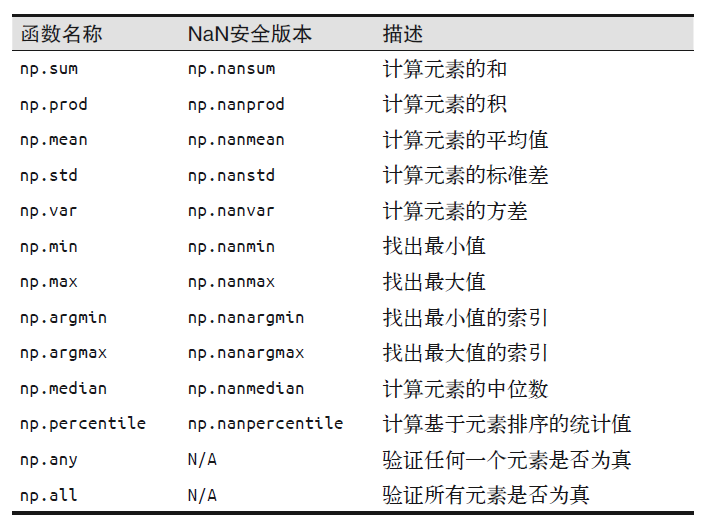
\includegraphics{HW4_1.png}
\caption{flow\_chart}
\end{figure}

    大多数的聚合都有对 NaN
值的安全处理策略(NaN-safe),即计算时忽略所有的缺失值。

    \begin{tcolorbox}[breakable, size=fbox, boxrule=1pt, pad at break*=1mm,colback=cellbackground, colframe=cellborder]
\prompt{In}{incolor}{72}{\boxspacing}
\begin{Verbatim}[commandchars=\\\{\}]
\PY{n}{big\PYZus{}array} \PY{o}{=} \PY{n}{np}\PY{o}{.}\PY{n}{random}\PY{o}{.}\PY{n}{rand}\PY{p}{(}\PY{l+m+mi}{1000000}\PY{p}{)}
\PY{n}{big\PYZus{}array}
\end{Verbatim}
\end{tcolorbox}

            \begin{tcolorbox}[breakable, size=fbox, boxrule=.5pt, pad at break*=1mm, opacityfill=0]
\prompt{Out}{outcolor}{72}{\boxspacing}
\begin{Verbatim}[commandchars=\\\{\}]
array([0.13073622, 0.6731387 , 0.59959097, {\ldots}, 0.04275875, 0.87771788,
       0.50653486])
\end{Verbatim}
\end{tcolorbox}
        
    \begin{tcolorbox}[breakable, size=fbox, boxrule=1pt, pad at break*=1mm,colback=cellbackground, colframe=cellborder]
\prompt{In}{incolor}{73}{\boxspacing}
\begin{Verbatim}[commandchars=\\\{\}]
\PY{n+nb}{min}\PY{p}{(}\PY{n}{big\PYZus{}array}\PY{p}{)}\PY{p}{,} \PY{n+nb}{max}\PY{p}{(}\PY{n}{big\PYZus{}array}\PY{p}{)}
\end{Verbatim}
\end{tcolorbox}

            \begin{tcolorbox}[breakable, size=fbox, boxrule=.5pt, pad at break*=1mm, opacityfill=0]
\prompt{Out}{outcolor}{73}{\boxspacing}
\begin{Verbatim}[commandchars=\\\{\}]
(3.958909644552477e-09, 0.9999997899162943)
\end{Verbatim}
\end{tcolorbox}
        
    在对较大的数据进行分析时,一项基本的工作就是有效的数据累计(summarization):计算累计(aggregation)指标,如sum()、mean()、median()、min()
和max(),其中每一个指 标都呈现了大数据集的特征。

    \begin{tcolorbox}[breakable, size=fbox, boxrule=1pt, pad at break*=1mm,colback=cellbackground, colframe=cellborder]
\prompt{In}{incolor}{79}{\boxspacing}
\begin{Verbatim}[commandchars=\\\{\}]
\PY{c+c1}{\PYZsh{} seaborn 行星数据中包含了截至2014 年已被发现的一千多颗外行星的资料。}
\PY{k+kn}{import} \PY{n+nn}{seaborn} \PY{k}{as} \PY{n+nn}{sns}
\PY{n}{planets} \PY{o}{=} \PY{n}{sns}\PY{o}{.}\PY{n}{load\PYZus{}dataset}\PY{p}{(}\PY{l+s+s1}{\PYZsq{}}\PY{l+s+s1}{planets}\PY{l+s+s1}{\PYZsq{}}\PY{p}{)}
\PY{n}{planets}\PY{o}{.}\PY{n}{shape}
\end{Verbatim}
\end{tcolorbox}

            \begin{tcolorbox}[breakable, size=fbox, boxrule=.5pt, pad at break*=1mm, opacityfill=0]
\prompt{Out}{outcolor}{79}{\boxspacing}
\begin{Verbatim}[commandchars=\\\{\}]
(1035, 6)
\end{Verbatim}
\end{tcolorbox}
        
    \begin{tcolorbox}[breakable, size=fbox, boxrule=1pt, pad at break*=1mm,colback=cellbackground, colframe=cellborder]
\prompt{In}{incolor}{76}{\boxspacing}
\begin{Verbatim}[commandchars=\\\{\}]
\PY{n}{planets}\PY{o}{.}\PY{n}{head}\PY{p}{(}\PY{p}{)}
\end{Verbatim}
\end{tcolorbox}

            \begin{tcolorbox}[breakable, size=fbox, boxrule=.5pt, pad at break*=1mm, opacityfill=0]
\prompt{Out}{outcolor}{76}{\boxspacing}
\begin{Verbatim}[commandchars=\\\{\}]
            method  number  orbital\_period   mass  distance  year
0  Radial Velocity       1         269.300   7.10     77.40  2006
1  Radial Velocity       1         874.774   2.21     56.95  2008
2  Radial Velocity       1         763.000   2.60     19.84  2011
3  Radial Velocity       1         326.030  19.40    110.62  2007
4  Radial Velocity       1         516.220  10.50    119.47  2009
\end{Verbatim}
\end{tcolorbox}
        
    与一维 NumPy 数组相同,Pandas 的 Series 的累计函数也会返回一个统计值:

    \begin{tcolorbox}[breakable, size=fbox, boxrule=1pt, pad at break*=1mm,colback=cellbackground, colframe=cellborder]
\prompt{In}{incolor}{80}{\boxspacing}
\begin{Verbatim}[commandchars=\\\{\}]
\PY{n}{rng} \PY{o}{=} \PY{n}{np}\PY{o}{.}\PY{n}{random}\PY{o}{.}\PY{n}{RandomState}\PY{p}{(}\PY{l+m+mi}{42}\PY{p}{)}
\PY{n}{ser} \PY{o}{=} \PY{n}{pd}\PY{o}{.}\PY{n}{Series}\PY{p}{(}\PY{n}{rng}\PY{o}{.}\PY{n}{rand}\PY{p}{(}\PY{l+m+mi}{5}\PY{p}{)}\PY{p}{)}
\PY{n}{ser}
\end{Verbatim}
\end{tcolorbox}

            \begin{tcolorbox}[breakable, size=fbox, boxrule=.5pt, pad at break*=1mm, opacityfill=0]
\prompt{Out}{outcolor}{80}{\boxspacing}
\begin{Verbatim}[commandchars=\\\{\}]
0    0.374540
1    0.950714
2    0.731994
3    0.598658
4    0.156019
dtype: float64
\end{Verbatim}
\end{tcolorbox}
        
    \begin{tcolorbox}[breakable, size=fbox, boxrule=1pt, pad at break*=1mm,colback=cellbackground, colframe=cellborder]
\prompt{In}{incolor}{81}{\boxspacing}
\begin{Verbatim}[commandchars=\\\{\}]
\PY{n}{ser}\PY{o}{.}\PY{n}{sum}\PY{p}{(}\PY{p}{)}
\end{Verbatim}
\end{tcolorbox}

            \begin{tcolorbox}[breakable, size=fbox, boxrule=.5pt, pad at break*=1mm, opacityfill=0]
\prompt{Out}{outcolor}{81}{\boxspacing}
\begin{Verbatim}[commandchars=\\\{\}]
2.811925491708157
\end{Verbatim}
\end{tcolorbox}
        
    \begin{tcolorbox}[breakable, size=fbox, boxrule=1pt, pad at break*=1mm,colback=cellbackground, colframe=cellborder]
\prompt{In}{incolor}{82}{\boxspacing}
\begin{Verbatim}[commandchars=\\\{\}]
\PY{n}{ser}\PY{o}{.}\PY{n}{mean}\PY{p}{(}\PY{p}{)}
\end{Verbatim}
\end{tcolorbox}

            \begin{tcolorbox}[breakable, size=fbox, boxrule=.5pt, pad at break*=1mm, opacityfill=0]
\prompt{Out}{outcolor}{82}{\boxspacing}
\begin{Verbatim}[commandchars=\\\{\}]
0.5623850983416314
\end{Verbatim}
\end{tcolorbox}
        
    DataFrame 的累计函数默认对每列进行统计:

    \begin{tcolorbox}[breakable, size=fbox, boxrule=1pt, pad at break*=1mm,colback=cellbackground, colframe=cellborder]
\prompt{In}{incolor}{83}{\boxspacing}
\begin{Verbatim}[commandchars=\\\{\}]
\PY{n}{df} \PY{o}{=} \PY{n}{pd}\PY{o}{.}\PY{n}{DataFrame}\PY{p}{(}\PY{p}{\PYZob{}}\PY{l+s+s1}{\PYZsq{}}\PY{l+s+s1}{A}\PY{l+s+s1}{\PYZsq{}}\PY{p}{:} \PY{n}{rng}\PY{o}{.}\PY{n}{rand}\PY{p}{(}\PY{l+m+mi}{5}\PY{p}{)}\PY{p}{,}\PY{l+s+s1}{\PYZsq{}}\PY{l+s+s1}{B}\PY{l+s+s1}{\PYZsq{}}\PY{p}{:} \PY{n}{rng}\PY{o}{.}\PY{n}{rand}\PY{p}{(}\PY{l+m+mi}{5}\PY{p}{)}\PY{p}{\PYZcb{}}\PY{p}{)}
\PY{n}{df}
\end{Verbatim}
\end{tcolorbox}

            \begin{tcolorbox}[breakable, size=fbox, boxrule=.5pt, pad at break*=1mm, opacityfill=0]
\prompt{Out}{outcolor}{83}{\boxspacing}
\begin{Verbatim}[commandchars=\\\{\}]
          A         B
0  0.155995  0.020584
1  0.058084  0.969910
2  0.866176  0.832443
3  0.601115  0.212339
4  0.708073  0.181825
\end{Verbatim}
\end{tcolorbox}
        
    \begin{tcolorbox}[breakable, size=fbox, boxrule=1pt, pad at break*=1mm,colback=cellbackground, colframe=cellborder]
\prompt{In}{incolor}{84}{\boxspacing}
\begin{Verbatim}[commandchars=\\\{\}]
\PY{n}{df}\PY{o}{.}\PY{n}{mean}\PY{p}{(}\PY{p}{)}
\end{Verbatim}
\end{tcolorbox}

            \begin{tcolorbox}[breakable, size=fbox, boxrule=.5pt, pad at break*=1mm, opacityfill=0]
\prompt{Out}{outcolor}{84}{\boxspacing}
\begin{Verbatim}[commandchars=\\\{\}]
A    0.477888
B    0.443420
dtype: float64
\end{Verbatim}
\end{tcolorbox}
        
    设置axis 参数,可以对每一行进行统计

    \begin{tcolorbox}[breakable, size=fbox, boxrule=1pt, pad at break*=1mm,colback=cellbackground, colframe=cellborder]
\prompt{In}{incolor}{85}{\boxspacing}
\begin{Verbatim}[commandchars=\\\{\}]
\PY{n}{df}\PY{o}{.}\PY{n}{mean}\PY{p}{(}\PY{n}{axis}\PY{o}{=}\PY{l+s+s1}{\PYZsq{}}\PY{l+s+s1}{columns}\PY{l+s+s1}{\PYZsq{}}\PY{p}{)}
\end{Verbatim}
\end{tcolorbox}

            \begin{tcolorbox}[breakable, size=fbox, boxrule=.5pt, pad at break*=1mm, opacityfill=0]
\prompt{Out}{outcolor}{85}{\boxspacing}
\begin{Verbatim}[commandchars=\\\{\}]
0    0.088290
1    0.513997
2    0.849309
3    0.406727
4    0.444949
dtype: float64
\end{Verbatim}
\end{tcolorbox}
        
    Pandas 的 Series 和 DataFrame 支持所有 Numpy
中介绍的常用累计函数。另外,还有一个非常方便的 describe()
方法可以计算每一列的若干常用统计值。让我们在行星数据上试验一
下,首先丢弃有缺失值的行:

    \begin{tcolorbox}[breakable, size=fbox, boxrule=1pt, pad at break*=1mm,colback=cellbackground, colframe=cellborder]
\prompt{In}{incolor}{86}{\boxspacing}
\begin{Verbatim}[commandchars=\\\{\}]
\PY{n}{planets}\PY{o}{.}\PY{n}{dropna}\PY{p}{(}\PY{p}{)}\PY{o}{.}\PY{n}{describe}\PY{p}{(}\PY{p}{)}
\end{Verbatim}
\end{tcolorbox}

            \begin{tcolorbox}[breakable, size=fbox, boxrule=.5pt, pad at break*=1mm, opacityfill=0]
\prompt{Out}{outcolor}{86}{\boxspacing}
\begin{Verbatim}[commandchars=\\\{\}]
          number  orbital\_period        mass    distance         year
count  498.00000      498.000000  498.000000  498.000000   498.000000
mean     1.73494      835.778671    2.509320   52.068213  2007.377510
std      1.17572     1469.128259    3.636274   46.596041     4.167284
min      1.00000        1.328300    0.003600    1.350000  1989.000000
25\%      1.00000       38.272250    0.212500   24.497500  2005.000000
50\%      1.00000      357.000000    1.245000   39.940000  2009.000000
75\%      2.00000      999.600000    2.867500   59.332500  2011.000000
max      6.00000    17337.500000   25.000000  354.000000  2014.000000
\end{Verbatim}
\end{tcolorbox}
        
    这是一种理解数据集所有统计属性的有效方法。例如,从年份 year
列中可以看出,1989年首次发现外行星,而且一半的已知外行星都是在 2010
年及以后的年份被发现的。这主要得益于开普勒计划------一个通过激光望远镜发现恒星周围椭圆轨道行星的太空计划。

    Pandas 内置的一些累计方法如图所示。

    \begin{figure}
\centering
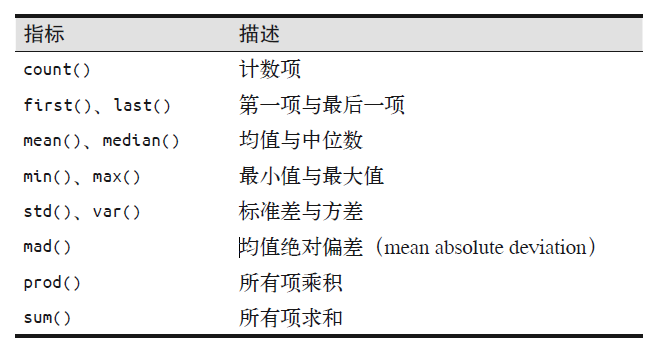
\includegraphics{HW4_2.png}
\caption{flow\_chart}
\end{figure}

    \hypertarget{groupbyux5206ux5272ux5e94ux7528ux548cux7ec4ux5408}{%
\subsection{GroupBy:分割、应用和组合}\label{groupbyux5206ux5272ux5e94ux7528ux548cux7ec4ux5408}}

    简单的累计方法可以让我们对数据集有一个笼统的认识,但是我们经常还需要对某些标签或索引的局部进行累计分析,这时就需要用到
groupby 了。虽然``分组''(group by)这个名字是借用 SQL
数据库语言的命令,但其理念引用发明 R 语言 frame 的 Hadley Wickham
的观点可能更合适:分割(split)、应用(apply)和组合(combine)。

    \begin{figure}
\centering
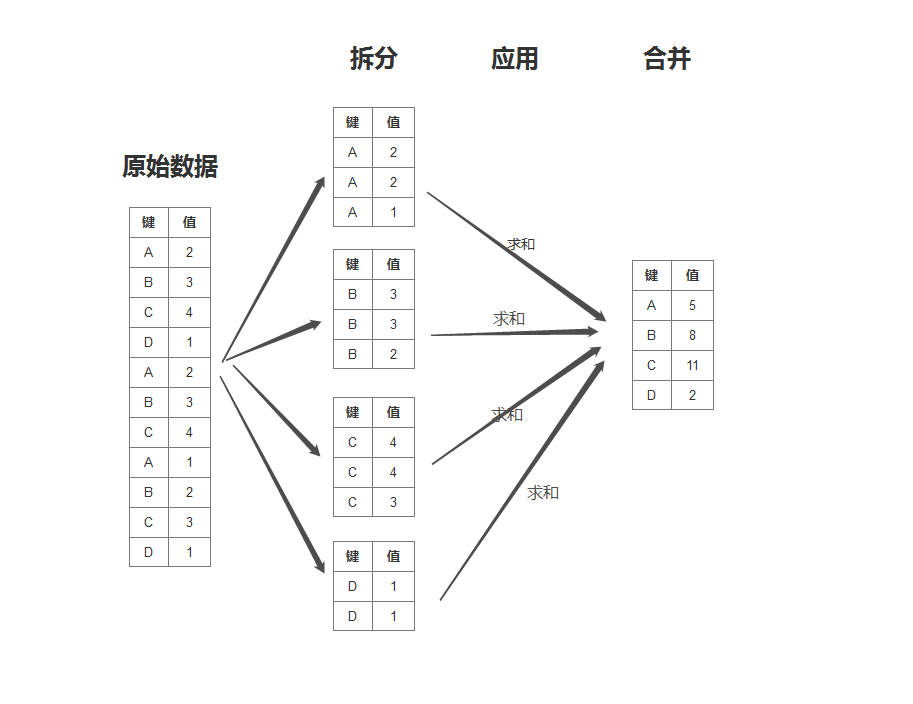
\includegraphics{hw4.png}
\caption{flow\_chart}
\end{figure}

    \begin{itemize}
\tightlist
\item
  分割步骤将 DataFrame 按照指定的键分割成若干组。
\item
  应用步骤对每个组应用函数,通常是累计、转换或过滤函数。
\item
  组合步骤将每一组的结果合并成一个输出数组。
\end{itemize}

    \begin{tcolorbox}[breakable, size=fbox, boxrule=1pt, pad at break*=1mm,colback=cellbackground, colframe=cellborder]
\prompt{In}{incolor}{92}{\boxspacing}
\begin{Verbatim}[commandchars=\\\{\}]
\PY{n}{data}\PY{o}{=}\PY{n}{pd}\PY{o}{.}\PY{n}{read\PYZus{}csv}\PY{p}{(}\PY{l+s+s2}{\PYZdq{}}\PY{l+s+s2}{hw4\PYZus{}data1.csv}\PY{l+s+s2}{\PYZdq{}}\PY{p}{,}\PY{n}{encoding}\PY{o}{=}\PY{l+s+s2}{\PYZdq{}}\PY{l+s+s2}{gbk}\PY{l+s+s2}{\PYZdq{}}\PY{p}{)}
\PY{n}{data}\PY{o}{.}\PY{n}{head}\PY{p}{(}\PY{p}{)}
\end{Verbatim}
\end{tcolorbox}

            \begin{tcolorbox}[breakable, size=fbox, boxrule=.5pt, pad at break*=1mm, opacityfill=0]
\prompt{Out}{outcolor}{92}{\boxspacing}
\begin{Verbatim}[commandchars=\\\{\}]
  CLASS\_ID  STD\_ID SUBJECT  SCORE  LAST\_SCORE
0    A1231       1      语文     97          94
1    A1231       1      数学    120         124
2    A1231       1      英语    107         109
3    A1231       1      生物     86          87
4    A1231       1      化学     92          88
\end{Verbatim}
\end{tcolorbox}
        
    假如对于上面的数据我们想要分科目查看平均分

    \begin{tcolorbox}[breakable, size=fbox, boxrule=1pt, pad at break*=1mm,colback=cellbackground, colframe=cellborder]
\prompt{In}{incolor}{93}{\boxspacing}
\begin{Verbatim}[commandchars=\\\{\}]
\PY{n}{group\PYZus{}sub}\PY{o}{=}\PY{n}{data}\PY{p}{[}\PY{l+s+s2}{\PYZdq{}}\PY{l+s+s2}{SCORE}\PY{l+s+s2}{\PYZdq{}}\PY{p}{]}\PY{o}{.}\PY{n}{groupby}\PY{p}{(}\PY{n}{data}\PY{p}{[}\PY{l+s+s2}{\PYZdq{}}\PY{l+s+s2}{SUBJECT}\PY{l+s+s2}{\PYZdq{}}\PY{p}{]}\PY{p}{)}
\PY{n}{group\PYZus{}sub}
\end{Verbatim}
\end{tcolorbox}

            \begin{tcolorbox}[breakable, size=fbox, boxrule=.5pt, pad at break*=1mm, opacityfill=0]
\prompt{Out}{outcolor}{93}{\boxspacing}
\begin{Verbatim}[commandchars=\\\{\}]
<pandas.core.groupby.generic.SeriesGroupBy object at 0x00000246063CF0C8>
\end{Verbatim}
\end{tcolorbox}
        
    这里的结果只是一个groupby对象,也就是我们指示图中的拆分,想要得到运算结果需要传入想要的函数

    \begin{tcolorbox}[breakable, size=fbox, boxrule=1pt, pad at break*=1mm,colback=cellbackground, colframe=cellborder]
\prompt{In}{incolor}{94}{\boxspacing}
\begin{Verbatim}[commandchars=\\\{\}]
\PY{n}{group\PYZus{}sub}\PY{o}{.}\PY{n}{mean}\PY{p}{(}\PY{p}{)}
\end{Verbatim}
\end{tcolorbox}

            \begin{tcolorbox}[breakable, size=fbox, boxrule=.5pt, pad at break*=1mm, opacityfill=0]
\prompt{Out}{outcolor}{94}{\boxspacing}
\begin{Verbatim}[commandchars=\\\{\}]
SUBJECT
化学     85.00
数学     98.50
物理     82.50
生物     82.50
英语    102.75
语文    100.00
Name: SCORE, dtype: float64
\end{Verbatim}
\end{tcolorbox}
        
    \begin{tcolorbox}[breakable, size=fbox, boxrule=1pt, pad at break*=1mm,colback=cellbackground, colframe=cellborder]
\prompt{In}{incolor}{95}{\boxspacing}
\begin{Verbatim}[commandchars=\\\{\}]
\PY{n}{group\PYZus{}sub}\PY{o}{.}\PY{n}{sum}\PY{p}{(}\PY{p}{)}
\end{Verbatim}
\end{tcolorbox}

            \begin{tcolorbox}[breakable, size=fbox, boxrule=.5pt, pad at break*=1mm, opacityfill=0]
\prompt{Out}{outcolor}{95}{\boxspacing}
\begin{Verbatim}[commandchars=\\\{\}]
SUBJECT
化学    340
数学    394
物理    330
生物    330
英语    411
语文    400
Name: SCORE, dtype: int64
\end{Verbatim}
\end{tcolorbox}
        
    如果既要分科目也要分班级的话

    \begin{tcolorbox}[breakable, size=fbox, boxrule=1pt, pad at break*=1mm,colback=cellbackground, colframe=cellborder]
\prompt{In}{incolor}{96}{\boxspacing}
\begin{Verbatim}[commandchars=\\\{\}]
\PY{n}{data}\PY{p}{[}\PY{l+s+s2}{\PYZdq{}}\PY{l+s+s2}{SCORE}\PY{l+s+s2}{\PYZdq{}}\PY{p}{]}\PY{o}{.}\PY{n}{groupby}\PY{p}{(}\PY{p}{[}\PY{n}{data}\PY{p}{[}\PY{l+s+s2}{\PYZdq{}}\PY{l+s+s2}{CLASS\PYZus{}ID}\PY{l+s+s2}{\PYZdq{}}\PY{p}{]}\PY{p}{,}\PY{n}{data}\PY{p}{[}\PY{l+s+s2}{\PYZdq{}}\PY{l+s+s2}{SUBJECT}\PY{l+s+s2}{\PYZdq{}}\PY{p}{]}\PY{p}{]}\PY{p}{)}\PY{o}{.}\PY{n}{mean}\PY{p}{(}\PY{p}{)}
\end{Verbatim}
\end{tcolorbox}

            \begin{tcolorbox}[breakable, size=fbox, boxrule=.5pt, pad at break*=1mm, opacityfill=0]
\prompt{Out}{outcolor}{96}{\boxspacing}
\begin{Verbatim}[commandchars=\\\{\}]
CLASS\_ID  SUBJECT
A1231     化学          80.0
          数学         109.0
          物理          77.0
          生物          82.5
          英语         114.0
          语文         101.5
A1232     化学          90.0
          数学          88.0
          物理          88.0
          生物          82.5
          英语          91.5
          语文          98.5
Name: SCORE, dtype: float64
\end{Verbatim}
\end{tcolorbox}
        
    GroupBy 对象的 aggregate()、filter()、transform() 和 apply()
方法,在数据组合之前实现了大量高效的操作。

    \begin{tcolorbox}[breakable, size=fbox, boxrule=1pt, pad at break*=1mm,colback=cellbackground, colframe=cellborder]
\prompt{In}{incolor}{97}{\boxspacing}
\begin{Verbatim}[commandchars=\\\{\}]
\PY{n}{rng} \PY{o}{=} \PY{n}{np}\PY{o}{.}\PY{n}{random}\PY{o}{.}\PY{n}{RandomState}\PY{p}{(}\PY{l+m+mi}{0}\PY{p}{)}
\PY{n}{df} \PY{o}{=} \PY{n}{pd}\PY{o}{.}\PY{n}{DataFrame}\PY{p}{(}\PY{p}{\PYZob{}}\PY{l+s+s1}{\PYZsq{}}\PY{l+s+s1}{key}\PY{l+s+s1}{\PYZsq{}}\PY{p}{:} \PY{p}{[}\PY{l+s+s1}{\PYZsq{}}\PY{l+s+s1}{A}\PY{l+s+s1}{\PYZsq{}}\PY{p}{,} \PY{l+s+s1}{\PYZsq{}}\PY{l+s+s1}{B}\PY{l+s+s1}{\PYZsq{}}\PY{p}{,} \PY{l+s+s1}{\PYZsq{}}\PY{l+s+s1}{C}\PY{l+s+s1}{\PYZsq{}}\PY{p}{,} \PY{l+s+s1}{\PYZsq{}}\PY{l+s+s1}{A}\PY{l+s+s1}{\PYZsq{}}\PY{p}{,} \PY{l+s+s1}{\PYZsq{}}\PY{l+s+s1}{B}\PY{l+s+s1}{\PYZsq{}}\PY{p}{,} \PY{l+s+s1}{\PYZsq{}}\PY{l+s+s1}{C}\PY{l+s+s1}{\PYZsq{}}\PY{p}{]}\PY{p}{,}\PY{l+s+s1}{\PYZsq{}}\PY{l+s+s1}{data1}\PY{l+s+s1}{\PYZsq{}}\PY{p}{:} \PY{n+nb}{range}\PY{p}{(}\PY{l+m+mi}{6}\PY{p}{)}\PY{p}{,}\PY{l+s+s1}{\PYZsq{}}\PY{l+s+s1}{data2}\PY{l+s+s1}{\PYZsq{}}\PY{p}{:} \PY{n}{rng}\PY{o}{.}\PY{n}{randint}\PY{p}{(}\PY{l+m+mi}{0}\PY{p}{,} \PY{l+m+mi}{10}\PY{p}{,} \PY{l+m+mi}{6}\PY{p}{)}\PY{p}{\PYZcb{}}\PY{p}{,}
                  \PY{n}{columns} \PY{o}{=} \PY{p}{[}\PY{l+s+s1}{\PYZsq{}}\PY{l+s+s1}{key}\PY{l+s+s1}{\PYZsq{}}\PY{p}{,} \PY{l+s+s1}{\PYZsq{}}\PY{l+s+s1}{data1}\PY{l+s+s1}{\PYZsq{}}\PY{p}{,} \PY{l+s+s1}{\PYZsq{}}\PY{l+s+s1}{data2}\PY{l+s+s1}{\PYZsq{}}\PY{p}{]}\PY{p}{)}
\PY{n}{df}
\end{Verbatim}
\end{tcolorbox}

            \begin{tcolorbox}[breakable, size=fbox, boxrule=.5pt, pad at break*=1mm, opacityfill=0]
\prompt{Out}{outcolor}{97}{\boxspacing}
\begin{Verbatim}[commandchars=\\\{\}]
  key  data1  data2
0   A      0      5
1   B      1      0
2   C      2      3
3   A      3      3
4   B      4      7
5   C      5      9
\end{Verbatim}
\end{tcolorbox}
        
    \textbf{累计}。我们目前比较熟悉的 GroupBy 累计方法只有 sum() 和 median()
之类的简单函数,但是 aggregate()
其实可以支持更复杂的操作,比如字符串、函数或者函数列表,并且能一次性计算所有累计值。

    \begin{tcolorbox}[breakable, size=fbox, boxrule=1pt, pad at break*=1mm,colback=cellbackground, colframe=cellborder]
\prompt{In}{incolor}{98}{\boxspacing}
\begin{Verbatim}[commandchars=\\\{\}]
\PY{n}{df}\PY{o}{.}\PY{n}{groupby}\PY{p}{(}\PY{l+s+s1}{\PYZsq{}}\PY{l+s+s1}{key}\PY{l+s+s1}{\PYZsq{}}\PY{p}{)}\PY{o}{.}\PY{n}{aggregate}\PY{p}{(}\PY{p}{[}\PY{l+s+s1}{\PYZsq{}}\PY{l+s+s1}{min}\PY{l+s+s1}{\PYZsq{}}\PY{p}{,} \PY{n}{np}\PY{o}{.}\PY{n}{median}\PY{p}{,} \PY{n+nb}{max}\PY{p}{]}\PY{p}{)}
\end{Verbatim}
\end{tcolorbox}

            \begin{tcolorbox}[breakable, size=fbox, boxrule=.5pt, pad at break*=1mm, opacityfill=0]
\prompt{Out}{outcolor}{98}{\boxspacing}
\begin{Verbatim}[commandchars=\\\{\}]
    data1            data2
      min median max   min median max
key
A       0    1.5   3     3    4.0   5
B       1    2.5   4     0    3.5   7
C       2    3.5   5     3    6.0   9
\end{Verbatim}
\end{tcolorbox}
        
    另一种用法就是通过Python 字典指定不同列需要累计的函数:

    \begin{tcolorbox}[breakable, size=fbox, boxrule=1pt, pad at break*=1mm,colback=cellbackground, colframe=cellborder]
\prompt{In}{incolor}{99}{\boxspacing}
\begin{Verbatim}[commandchars=\\\{\}]
\PY{n}{df}\PY{o}{.}\PY{n}{groupby}\PY{p}{(}\PY{l+s+s1}{\PYZsq{}}\PY{l+s+s1}{key}\PY{l+s+s1}{\PYZsq{}}\PY{p}{)}\PY{o}{.}\PY{n}{aggregate}\PY{p}{(}\PY{p}{\PYZob{}}\PY{l+s+s1}{\PYZsq{}}\PY{l+s+s1}{data1}\PY{l+s+s1}{\PYZsq{}}\PY{p}{:} \PY{l+s+s1}{\PYZsq{}}\PY{l+s+s1}{min}\PY{l+s+s1}{\PYZsq{}}\PY{p}{,}\PY{l+s+s1}{\PYZsq{}}\PY{l+s+s1}{data2}\PY{l+s+s1}{\PYZsq{}}\PY{p}{:} \PY{l+s+s1}{\PYZsq{}}\PY{l+s+s1}{max}\PY{l+s+s1}{\PYZsq{}}\PY{p}{\PYZcb{}}\PY{p}{)}
\end{Verbatim}
\end{tcolorbox}

            \begin{tcolorbox}[breakable, size=fbox, boxrule=.5pt, pad at break*=1mm, opacityfill=0]
\prompt{Out}{outcolor}{99}{\boxspacing}
\begin{Verbatim}[commandchars=\\\{\}]
     data1  data2
key
A        0      5
B        1      7
C        2      9
\end{Verbatim}
\end{tcolorbox}
        
    \textbf{过滤}。过滤操作可以让你按照分组的属性丢弃若干数据。例如,我们可能只需要保留标准差超过某个阈值的组:

    \begin{tcolorbox}[breakable, size=fbox, boxrule=1pt, pad at break*=1mm,colback=cellbackground, colframe=cellborder]
\prompt{In}{incolor}{101}{\boxspacing}
\begin{Verbatim}[commandchars=\\\{\}]
\PY{k}{def} \PY{n+nf}{filter\PYZus{}func}\PY{p}{(}\PY{n}{x}\PY{p}{)}\PY{p}{:}
    \PY{k}{return} \PY{n}{x}\PY{p}{[}\PY{l+s+s1}{\PYZsq{}}\PY{l+s+s1}{data2}\PY{l+s+s1}{\PYZsq{}}\PY{p}{]}\PY{o}{.}\PY{n}{std}\PY{p}{(}\PY{p}{)} \PY{o}{\PYZgt{}} \PY{l+m+mi}{4}
\PY{n}{df} 
\end{Verbatim}
\end{tcolorbox}

            \begin{tcolorbox}[breakable, size=fbox, boxrule=.5pt, pad at break*=1mm, opacityfill=0]
\prompt{Out}{outcolor}{101}{\boxspacing}
\begin{Verbatim}[commandchars=\\\{\}]
  key  data1  data2
0   A      0      5
1   B      1      0
2   C      2      3
3   A      3      3
4   B      4      7
5   C      5      9
\end{Verbatim}
\end{tcolorbox}
        
    \begin{tcolorbox}[breakable, size=fbox, boxrule=1pt, pad at break*=1mm,colback=cellbackground, colframe=cellborder]
\prompt{In}{incolor}{102}{\boxspacing}
\begin{Verbatim}[commandchars=\\\{\}]
\PY{n}{df}\PY{o}{.}\PY{n}{groupby}\PY{p}{(}\PY{l+s+s1}{\PYZsq{}}\PY{l+s+s1}{key}\PY{l+s+s1}{\PYZsq{}}\PY{p}{)}\PY{o}{.}\PY{n}{std}\PY{p}{(}\PY{p}{)}
\end{Verbatim}
\end{tcolorbox}

            \begin{tcolorbox}[breakable, size=fbox, boxrule=.5pt, pad at break*=1mm, opacityfill=0]
\prompt{Out}{outcolor}{102}{\boxspacing}
\begin{Verbatim}[commandchars=\\\{\}]
       data1     data2
key
A    2.12132  1.414214
B    2.12132  4.949747
C    2.12132  4.242641
\end{Verbatim}
\end{tcolorbox}
        
    \begin{tcolorbox}[breakable, size=fbox, boxrule=1pt, pad at break*=1mm,colback=cellbackground, colframe=cellborder]
\prompt{In}{incolor}{103}{\boxspacing}
\begin{Verbatim}[commandchars=\\\{\}]
\PY{n}{df}\PY{o}{.}\PY{n}{groupby}\PY{p}{(}\PY{l+s+s1}{\PYZsq{}}\PY{l+s+s1}{key}\PY{l+s+s1}{\PYZsq{}}\PY{p}{)}\PY{o}{.}\PY{n}{filter}\PY{p}{(}\PY{n}{filter\PYZus{}func}\PY{p}{)}
\end{Verbatim}
\end{tcolorbox}

            \begin{tcolorbox}[breakable, size=fbox, boxrule=.5pt, pad at break*=1mm, opacityfill=0]
\prompt{Out}{outcolor}{103}{\boxspacing}
\begin{Verbatim}[commandchars=\\\{\}]
  key  data1  data2
1   B      1      0
2   C      2      3
4   B      4      7
5   C      5      9
\end{Verbatim}
\end{tcolorbox}
        
    filter() 函数会返回一个布尔值,表示每个组是否通过过滤。由于 A 组 `data2'
列的标准差不大于4,所以被丢弃了。

    \textbf{转换}。累计操作返回的是对组内全量数据缩减过的结果,而转换操作会返回一个新的全量数据。数据经过转换之后,其形状与原来的输入数据是一样的。常见的例子就是将每
一组的样本数据减去各组的均值,实现数据标准化:

    \begin{tcolorbox}[breakable, size=fbox, boxrule=1pt, pad at break*=1mm,colback=cellbackground, colframe=cellborder]
\prompt{In}{incolor}{104}{\boxspacing}
\begin{Verbatim}[commandchars=\\\{\}]
\PY{n}{df}\PY{o}{.}\PY{n}{groupby}\PY{p}{(}\PY{l+s+s1}{\PYZsq{}}\PY{l+s+s1}{key}\PY{l+s+s1}{\PYZsq{}}\PY{p}{)}\PY{o}{.}\PY{n}{transform}\PY{p}{(}\PY{k}{lambda} \PY{n}{x}\PY{p}{:} \PY{n}{x} \PY{o}{\PYZhy{}} \PY{n}{x}\PY{o}{.}\PY{n}{mean}\PY{p}{(}\PY{p}{)}\PY{p}{)}
\end{Verbatim}
\end{tcolorbox}

            \begin{tcolorbox}[breakable, size=fbox, boxrule=.5pt, pad at break*=1mm, opacityfill=0]
\prompt{Out}{outcolor}{104}{\boxspacing}
\begin{Verbatim}[commandchars=\\\{\}]
   data1  data2
0   -1.5    1.0
1   -1.5   -3.5
2   -1.5   -3.0
3    1.5   -1.0
4    1.5    3.5
5    1.5    3.0
\end{Verbatim}
\end{tcolorbox}
        
    \textbf{apply() 方法}。apply()
方法让你可以在每个组上应用任意方法。这个函数输入一个 DataFrame,返回一个
Pandas 对象(DataFrame
或Series)或一个标量(scalar,单个数值)。组合操作会适应返回结果类型。

    \begin{tcolorbox}[breakable, size=fbox, boxrule=1pt, pad at break*=1mm,colback=cellbackground, colframe=cellborder]
\prompt{In}{incolor}{105}{\boxspacing}
\begin{Verbatim}[commandchars=\\\{\}]
\PY{c+c1}{\PYZsh{} 将第一列数据以第二列的和为基数进行标准化}
\PY{k}{def} \PY{n+nf}{norm\PYZus{}by\PYZus{}data2}\PY{p}{(}\PY{n}{x}\PY{p}{)}\PY{p}{:}
    \PY{c+c1}{\PYZsh{} x是一个分组数据的DataFrame}
    \PY{n}{x}\PY{p}{[}\PY{l+s+s1}{\PYZsq{}}\PY{l+s+s1}{data1}\PY{l+s+s1}{\PYZsq{}}\PY{p}{]} \PY{o}{/}\PY{o}{=} \PY{n}{x}\PY{p}{[}\PY{l+s+s1}{\PYZsq{}}\PY{l+s+s1}{data2}\PY{l+s+s1}{\PYZsq{}}\PY{p}{]}\PY{o}{.}\PY{n}{sum}\PY{p}{(}\PY{p}{)}
    \PY{k}{return} \PY{n}{x}
\PY{n}{df}\PY{o}{.}\PY{n}{groupby}\PY{p}{(}\PY{l+s+s1}{\PYZsq{}}\PY{l+s+s1}{key}\PY{l+s+s1}{\PYZsq{}}\PY{p}{)}\PY{o}{.}\PY{n}{apply}\PY{p}{(}\PY{n}{norm\PYZus{}by\PYZus{}data2}\PY{p}{)}
\end{Verbatim}
\end{tcolorbox}

            \begin{tcolorbox}[breakable, size=fbox, boxrule=.5pt, pad at break*=1mm, opacityfill=0]
\prompt{Out}{outcolor}{105}{\boxspacing}
\begin{Verbatim}[commandchars=\\\{\}]
  key     data1  data2
0   A  0.000000      5
1   B  0.142857      0
2   C  0.166667      3
3   A  0.375000      3
4   B  0.571429      7
5   C  0.416667      9
\end{Verbatim}
\end{tcolorbox}
        
    GroupBy 里的 apply()
方法非常灵活,唯一需要注意的地方是它总是输入分组数据的 DataFrame,返回
Pandas 对象或标量。具体如何选择需要视情况而定。

    \hypertarget{knn-model}{%
\section{KNN Model}\label{knn-model}}

    \begin{tcolorbox}[breakable, size=fbox, boxrule=1pt, pad at break*=1mm,colback=cellbackground, colframe=cellborder]
\prompt{In}{incolor}{139}{\boxspacing}
\begin{Verbatim}[commandchars=\\\{\}]
\PY{n}{data}\PY{o}{=}\PY{n}{pd}\PY{o}{.}\PY{n}{read\PYZus{}csv}\PY{p}{(}\PY{l+s+s2}{\PYZdq{}}\PY{l+s+s2}{HW4\PYZus{}DATA2.csv}\PY{l+s+s2}{\PYZdq{}}\PY{p}{,}\PY{n}{index\PYZus{}col}\PY{o}{=}\PY{l+s+s2}{\PYZdq{}}\PY{l+s+s2}{index}\PY{l+s+s2}{\PYZdq{}}\PY{p}{)}
\PY{n}{data}
\end{Verbatim}
\end{tcolorbox}

            \begin{tcolorbox}[breakable, size=fbox, boxrule=.5pt, pad at break*=1mm, opacityfill=0]
\prompt{Out}{outcolor}{139}{\boxspacing}
\begin{Verbatim}[commandchars=\\\{\}]
       Sepal.Length  Sepal.Width  Pepal.Length  Pepal.Width     Species
index
1               5.1          3.5           1.4          0.2      setosa
2               4.9          3.0           1.4          0.2      setosa
3               4.7          3.2           1.3          0.2      setosa
4               4.6          3.1           1.5          0.2      setosa
48              4.6          3.2           1.4          0.2      setosa
49              5.3          3.7           1.5          0.2      setosa
50              5.0          3.3           1.4          0.2      setosa
51              7.0          3.2           4.7          1.4  versicolor
52              6.4          3.2           4.5          1.5  versicolor
53              6.9          3.1           4.9          1.5  versicolor
59              6.6          2.9           4.6          1.3  versicolor
118             7.7          3.8           6.7          2.2   virginica
119             7.7          2.6           6.9          2.3   virginica
\end{Verbatim}
\end{tcolorbox}
        
    \begin{tcolorbox}[breakable, size=fbox, boxrule=1pt, pad at break*=1mm,colback=cellbackground, colframe=cellborder]
\prompt{In}{incolor}{140}{\boxspacing}
\begin{Verbatim}[commandchars=\\\{\}]
\PY{n}{labels}\PY{o}{=}\PY{n}{data}\PY{o}{.}\PY{n}{pop}\PY{p}{(}\PY{l+s+s2}{\PYZdq{}}\PY{l+s+s2}{Species}\PY{l+s+s2}{\PYZdq{}}\PY{p}{)}
\PY{n}{labels}\PY{o}{=}\PY{n}{np}\PY{o}{.}\PY{n}{array}\PY{p}{(}\PY{n}{labels}\PY{p}{)}
\PY{n}{labels}
\end{Verbatim}
\end{tcolorbox}

            \begin{tcolorbox}[breakable, size=fbox, boxrule=.5pt, pad at break*=1mm, opacityfill=0]
\prompt{Out}{outcolor}{140}{\boxspacing}
\begin{Verbatim}[commandchars=\\\{\}]
array(['setosa', 'setosa', 'setosa', 'setosa', 'setosa', 'setosa',
       'setosa', 'versicolor', 'versicolor', 'versicolor', 'versicolor',
       'virginica', 'virginica'], dtype=object)
\end{Verbatim}
\end{tcolorbox}
        
    \begin{tcolorbox}[breakable, size=fbox, boxrule=1pt, pad at break*=1mm,colback=cellbackground, colframe=cellborder]
\prompt{In}{incolor}{141}{\boxspacing}
\begin{Verbatim}[commandchars=\\\{\}]
\PY{c+c1}{\PYZsh{}print(type(data.loc[1,:]))}
\PY{n}{data}\PY{o}{=}\PY{n}{np}\PY{o}{.}\PY{n}{array}\PY{p}{(}\PY{n}{data}\PY{p}{)}
\PY{n}{data}
\end{Verbatim}
\end{tcolorbox}

            \begin{tcolorbox}[breakable, size=fbox, boxrule=.5pt, pad at break*=1mm, opacityfill=0]
\prompt{Out}{outcolor}{141}{\boxspacing}
\begin{Verbatim}[commandchars=\\\{\}]
array([[5.1, 3.5, 1.4, 0.2],
       [4.9, 3. , 1.4, 0.2],
       [4.7, 3.2, 1.3, 0.2],
       [4.6, 3.1, 1.5, 0.2],
       [4.6, 3.2, 1.4, 0.2],
       [5.3, 3.7, 1.5, 0.2],
       [5. , 3.3, 1.4, 0.2],
       [7. , 3.2, 4.7, 1.4],
       [6.4, 3.2, 4.5, 1.5],
       [6.9, 3.1, 4.9, 1.5],
       [6.6, 2.9, 4.6, 1.3],
       [7.7, 3.8, 6.7, 2.2],
       [7.7, 2.6, 6.9, 2.3]])
\end{Verbatim}
\end{tcolorbox}
        
    \begin{tcolorbox}[breakable, size=fbox, boxrule=1pt, pad at break*=1mm,colback=cellbackground, colframe=cellborder]
\prompt{In}{incolor}{145}{\boxspacing}
\begin{Verbatim}[commandchars=\\\{\}]
\PY{k+kn}{from} \PY{n+nn}{numpy} \PY{k}{import} \PY{o}{*}
\PY{n}{new\PYZus{}t}\PY{o}{=}\PY{n}{np}\PY{o}{.}\PY{n}{array}\PY{p}{(}\PY{p}{[}\PY{l+m+mf}{6.3}\PY{p}{,}\PY{l+m+mf}{3.1}\PY{p}{,}\PY{l+m+mf}{4.8}\PY{p}{,}\PY{l+m+mf}{1.4}\PY{p}{]}\PY{p}{)}

\PY{n}{numSamples} \PY{o}{=} \PY{n}{data}\PY{o}{.}\PY{n}{shape}\PY{p}{[}\PY{l+m+mi}{0}\PY{p}{]}
\PY{n}{diff}\PY{o}{=}\PY{n}{tile}\PY{p}{(}\PY{n}{new\PYZus{}t}\PY{p}{,}\PY{p}{(}\PY{n}{numSamples}\PY{p}{,}\PY{l+m+mi}{1}\PY{p}{)}\PY{p}{)}\PY{o}{\PYZhy{}}\PY{n}{data}
\PY{n}{squreDiff} \PY{o}{=} \PY{n}{diff}\PY{o}{*}\PY{o}{*}\PY{l+m+mi}{2}
\PY{n}{squreDist} \PY{o}{=} \PY{n+nb}{sum}\PY{p}{(}\PY{n}{squreDiff}\PY{p}{,} \PY{n}{axis}\PY{o}{=}\PY{l+m+mi}{1}\PY{p}{)}
\PY{n}{distance} \PY{o}{=} \PY{n}{squreDist} \PY{o}{*}\PY{o}{*} \PY{l+m+mf}{0.5}
\PY{n}{distance}
\end{Verbatim}
\end{tcolorbox}

            \begin{tcolorbox}[breakable, size=fbox, boxrule=.5pt, pad at break*=1mm, opacityfill=0]
\prompt{Out}{outcolor}{145}{\boxspacing}
\begin{Verbatim}[commandchars=\\\{\}]
array([3.82099463, 3.86910842, 4.03236903, 3.90128184, 3.98748041,
       3.7       , 3.83796821, 0.71414284, 0.34641016, 0.6164414 ,
       0.42426407, 2.58843582, 2.72580263])
\end{Verbatim}
\end{tcolorbox}
        
    \begin{tcolorbox}[breakable, size=fbox, boxrule=1pt, pad at break*=1mm,colback=cellbackground, colframe=cellborder]
\prompt{In}{incolor}{148}{\boxspacing}
\begin{Verbatim}[commandchars=\\\{\}]
\PY{n}{sortedDistIndices} \PY{o}{=} \PY{n}{argsort}\PY{p}{(}\PY{n}{distance}\PY{p}{)}
\PY{n}{sortedDistIndices}
\end{Verbatim}
\end{tcolorbox}

            \begin{tcolorbox}[breakable, size=fbox, boxrule=.5pt, pad at break*=1mm, opacityfill=0]
\prompt{Out}{outcolor}{148}{\boxspacing}
\begin{Verbatim}[commandchars=\\\{\}]
array([ 8, 10,  9,  7, 11, 12,  5,  0,  6,  1,  3,  4,  2], dtype=int64)
\end{Verbatim}
\end{tcolorbox}
        
    \begin{tcolorbox}[breakable, size=fbox, boxrule=1pt, pad at break*=1mm,colback=cellbackground, colframe=cellborder]
\prompt{In}{incolor}{154}{\boxspacing}
\begin{Verbatim}[commandchars=\\\{\}]
\PY{n}{classCount} \PY{o}{=} \PY{p}{\PYZob{}}\PY{p}{\PYZcb{}}
\PY{n}{K} \PY{o}{=} \PY{l+m+mi}{4}
\PY{k}{for} \PY{n}{i} \PY{o+ow}{in} \PY{n+nb}{range}\PY{p}{(}\PY{n}{K}\PY{p}{)}\PY{p}{:}
    \PY{n}{voteLabel} \PY{o}{=} \PY{n}{labels}\PY{p}{[}\PY{n}{sortedDistIndices}\PY{p}{[}\PY{n}{i}\PY{p}{]}\PY{p}{]}
    \PY{n+nb}{print}\PY{p}{(}\PY{n}{voteLabel}\PY{p}{)}
    \PY{n}{classCount}\PY{p}{[}\PY{n}{voteLabel}\PY{p}{]} \PY{o}{=} \PY{n}{classCount}\PY{o}{.}\PY{n}{get}\PY{p}{(}\PY{n}{voteLabel}\PY{p}{,} \PY{l+m+mi}{0}\PY{p}{)} \PY{o}{+} \PY{l+m+mi}{1}
\PY{n+nb}{print}\PY{p}{(}\PY{n}{classCount}\PY{p}{)}

\PY{n}{maxCount} \PY{o}{=} \PY{l+m+mi}{0}
\PY{k}{for} \PY{n}{k}\PY{p}{,} \PY{n}{v} \PY{o+ow}{in} \PY{n}{classCount}\PY{o}{.}\PY{n}{items}\PY{p}{(}\PY{p}{)}\PY{p}{:}
    \PY{k}{if} \PY{n}{v} \PY{o}{\PYZgt{}} \PY{n}{maxCount}\PY{p}{:}
        \PY{n}{maxCount} \PY{o}{=} \PY{n}{v}
        \PY{n}{maxIndex} \PY{o}{=} \PY{n}{k}

\PY{n+nb}{print}\PY{p}{(}\PY{l+s+s2}{\PYZdq{}}\PY{l+s+s2}{Your input is:}\PY{l+s+s2}{\PYZdq{}}\PY{p}{,} \PY{n}{new\PYZus{}t}\PY{p}{,} \PY{l+s+s2}{\PYZdq{}}\PY{l+s+s2}{and classified to class: }\PY{l+s+s2}{\PYZdq{}}\PY{p}{,} \PY{n}{maxIndex}\PY{p}{)}
\end{Verbatim}
\end{tcolorbox}

    \begin{Verbatim}[commandchars=\\\{\}]
versicolor
versicolor
versicolor
versicolor
\{'versicolor': 4\}
Your input is: [6.3 3.1 4.8 1.4] and classified to class:  versicolor
    \end{Verbatim}

    \hypertarget{ux66fcux54c8ux987fux8dddux79bbmanhattan-distance}{%
\section{曼哈顿距离((Manhattan
Distance))}\label{ux66fcux54c8ux987fux8dddux79bbmanhattan-distance}}

    \[d(x,y)=\sqrt{\sum\limits_{k=1}^n|x_k-y_k|}\]

    \begin{tcolorbox}[breakable, size=fbox, boxrule=1pt, pad at break*=1mm,colback=cellbackground, colframe=cellborder]
\prompt{In}{incolor}{167}{\boxspacing}
\begin{Verbatim}[commandchars=\\\{\}]
\PY{k+kn}{import} \PY{n+nn}{matplotlib}\PY{n+nn}{.}\PY{n+nn}{pyplot} \PY{k}{as} \PY{n+nn}{plt}
\PY{k+kn}{from} \PY{n+nn}{mpl\PYZus{}toolkits}\PY{n+nn}{.}\PY{n+nn}{mplot3d} \PY{k}{import} \PY{n}{Axes3D}
\PY{k+kn}{from} \PY{n+nn}{mpl\PYZus{}toolkits}\PY{n+nn}{.}\PY{n+nn}{mplot3d} \PY{k}{import} \PY{n}{proj3d}
\PY{k+kn}{import} \PY{n+nn}{math}
\PY{k}{def} \PY{n+nf}{Manhattan\PYZus{}Dist}\PY{p}{(}\PY{n}{X}\PY{p}{,}\PY{n}{Y}\PY{p}{)}\PY{p}{:}
    \PY{k}{return} \PY{n}{math}\PY{o}{.}\PY{n}{sqrt}\PY{p}{(}\PY{n+nb}{sum}\PY{p}{(}\PY{p}{[}\PY{n+nb}{abs}\PY{p}{(}\PY{n}{x}\PY{o}{\PYZhy{}}\PY{n}{y}\PY{p}{)} \PY{k}{for} \PY{p}{(}\PY{n}{x}\PY{p}{,}\PY{n}{y}\PY{p}{)} \PY{o+ow}{in} \PY{n+nb}{zip}\PY{p}{(}\PY{n}{X}\PY{p}{,}\PY{n}{Y}\PY{p}{)}\PY{p}{]}\PY{p}{)}\PY{p}{)}
\end{Verbatim}
\end{tcolorbox}

    \begin{tcolorbox}[breakable, size=fbox, boxrule=1pt, pad at break*=1mm,colback=cellbackground, colframe=cellborder]
\prompt{In}{incolor}{190}{\boxspacing}
\begin{Verbatim}[commandchars=\\\{\}]
\PY{n}{X}\PY{o}{=}\PY{p}{[}\PY{l+m+mi}{1}\PY{p}{,}\PY{l+m+mi}{2}\PY{p}{,}\PY{l+m+mi}{3}\PY{p}{]}
\PY{n}{Y}\PY{o}{=}\PY{p}{[}\PY{l+m+mi}{0}\PY{p}{,}\PY{l+m+mi}{1}\PY{p}{,}\PY{l+m+mi}{2}\PY{p}{]}
\end{Verbatim}
\end{tcolorbox}

    \begin{tcolorbox}[breakable, size=fbox, boxrule=1pt, pad at break*=1mm,colback=cellbackground, colframe=cellborder]
\prompt{In}{incolor}{164}{\boxspacing}
\begin{Verbatim}[commandchars=\\\{\}]
\PY{n}{Manhattan\PYZus{}Dist}\PY{p}{(}\PY{n}{X}\PY{p}{,}\PY{n}{Y}\PY{p}{)}
\end{Verbatim}
\end{tcolorbox}

            \begin{tcolorbox}[breakable, size=fbox, boxrule=.5pt, pad at break*=1mm, opacityfill=0]
\prompt{Out}{outcolor}{164}{\boxspacing}
\begin{Verbatim}[commandchars=\\\{\}]
1.7320508075688772
\end{Verbatim}
\end{tcolorbox}
        
    \begin{tcolorbox}[breakable, size=fbox, boxrule=1pt, pad at break*=1mm,colback=cellbackground, colframe=cellborder]
\prompt{In}{incolor}{170}{\boxspacing}
\begin{Verbatim}[commandchars=\\\{\}]
\PY{n}{fig}\PY{o}{=}\PY{n}{plt}\PY{o}{.}\PY{n}{figure}\PY{p}{(}\PY{n}{figsize}\PY{o}{=}\PY{p}{(}\PY{l+m+mi}{7}\PY{p}{,}\PY{l+m+mi}{7}\PY{p}{)}\PY{p}{)}
\PY{n}{ax}\PY{o}{=}\PY{n}{fig}\PY{o}{.}\PY{n}{add\PYZus{}subplot}\PY{p}{(}\PY{l+m+mi}{111}\PY{p}{,}\PY{n}{projection}\PY{o}{=}\PY{l+s+s1}{\PYZsq{}}\PY{l+s+s1}{3d}\PY{l+s+s1}{\PYZsq{}}\PY{p}{)}
\PY{n}{ax}\PY{o}{.}\PY{n}{scatter}\PY{p}{(}\PY{p}{(}\PY{n}{X}\PY{p}{[}\PY{l+m+mi}{0}\PY{p}{]}\PY{p}{,}\PY{n}{Y}\PY{p}{[}\PY{l+m+mi}{0}\PY{p}{]}\PY{p}{)}\PY{p}{,}\PY{p}{(}\PY{n}{X}\PY{p}{[}\PY{l+m+mi}{1}\PY{p}{]}\PY{p}{,}\PY{n}{Y}\PY{p}{[}\PY{l+m+mi}{1}\PY{p}{]}\PY{p}{)}\PY{p}{,}\PY{p}{(}\PY{n}{X}\PY{p}{[}\PY{l+m+mi}{2}\PY{p}{]}\PY{p}{,}\PY{n}{Y}\PY{p}{[}\PY{l+m+mi}{2}\PY{p}{]}\PY{p}{)}\PY{p}{,}\PY{n}{color}\PY{o}{=}\PY{l+s+s1}{\PYZsq{}}\PY{l+s+s1}{b}\PY{l+s+s1}{\PYZsq{}}\PY{p}{,}\PY{n}{s}\PY{o}{=}\PY{l+m+mi}{50}\PY{p}{)}
\PY{n}{ax}\PY{o}{.}\PY{n}{plot}\PY{p}{(}\PY{p}{(}\PY{n}{X}\PY{p}{[}\PY{l+m+mi}{0}\PY{p}{]}\PY{p}{,}\PY{n}{Y}\PY{p}{[}\PY{l+m+mi}{0}\PY{p}{]}\PY{p}{)}\PY{p}{,}\PY{p}{(}\PY{n}{X}\PY{p}{[}\PY{l+m+mi}{1}\PY{p}{]}\PY{p}{,}\PY{n}{Y}\PY{p}{[}\PY{l+m+mi}{1}\PY{p}{]}\PY{p}{)}\PY{p}{,}\PY{p}{(}\PY{n}{X}\PY{p}{[}\PY{l+m+mi}{2}\PY{p}{]}\PY{p}{,}\PY{n}{Y}\PY{p}{[}\PY{l+m+mi}{2}\PY{p}{]}\PY{p}{)}\PY{p}{,}\PY{n}{color}\PY{o}{=}\PY{l+s+s1}{\PYZsq{}}\PY{l+s+s1}{r}\PY{l+s+s1}{\PYZsq{}}\PY{p}{)}
\end{Verbatim}
\end{tcolorbox}

            \begin{tcolorbox}[breakable, size=fbox, boxrule=.5pt, pad at break*=1mm, opacityfill=0]
\prompt{Out}{outcolor}{170}{\boxspacing}
\begin{Verbatim}[commandchars=\\\{\}]
[<mpl\_toolkits.mplot3d.art3d.Line3D at 0x2460d044748>]
\end{Verbatim}
\end{tcolorbox}
        
    \begin{center}
    \adjustimage{max size={0.9\linewidth}{0.9\paperheight}}{output_123_1.png}
    \end{center}
    { \hspace*{\fill} \\}
    
    \hypertarget{ux5207ux6bd4ux96eaux592bux8dddux79bbchebyshev-distance}{%
\section{切比雪夫距离(Chebyshev
Distance)}\label{ux5207ux6bd4ux96eaux592bux8dddux79bbchebyshev-distance}}

    \[d(x,y)=\max\limits_{k=1}^n|x_k-y_k|\]

    \begin{tcolorbox}[breakable, size=fbox, boxrule=1pt, pad at break*=1mm,colback=cellbackground, colframe=cellborder]
\prompt{In}{incolor}{171}{\boxspacing}
\begin{Verbatim}[commandchars=\\\{\}]
\PY{k}{def} \PY{n+nf}{Chebyshev\PYZus{}Dist}\PY{p}{(}\PY{n}{X}\PY{p}{,}\PY{n}{Y}\PY{p}{)}\PY{p}{:}
    \PY{k}{return} \PY{n+nb}{max}\PY{p}{(}\PY{p}{[}\PY{n+nb}{abs}\PY{p}{(}\PY{n}{x}\PY{o}{\PYZhy{}}\PY{n}{y}\PY{p}{)} \PY{k}{for} \PY{p}{(}\PY{n}{x}\PY{p}{,}\PY{n}{y}\PY{p}{)} \PY{o+ow}{in} \PY{n+nb}{zip}\PY{p}{(}\PY{n}{X}\PY{p}{,}\PY{n}{Y}\PY{p}{)}\PY{p}{]}\PY{p}{)}
\end{Verbatim}
\end{tcolorbox}

    \begin{tcolorbox}[breakable, size=fbox, boxrule=1pt, pad at break*=1mm,colback=cellbackground, colframe=cellborder]
\prompt{In}{incolor}{175}{\boxspacing}
\begin{Verbatim}[commandchars=\\\{\}]
\PY{n}{Chebyshev\PYZus{}Dist}\PY{p}{(}\PY{n}{X}\PY{p}{,}\PY{n}{Y}\PY{p}{)}
\end{Verbatim}
\end{tcolorbox}

            \begin{tcolorbox}[breakable, size=fbox, boxrule=.5pt, pad at break*=1mm, opacityfill=0]
\prompt{Out}{outcolor}{175}{\boxspacing}
\begin{Verbatim}[commandchars=\\\{\}]
1
\end{Verbatim}
\end{tcolorbox}
        
    \hypertarget{ux95f5ux53efux592bux65afux57faux8dddux79bbminkowski-distance}{%
\section{闵可夫斯基距离(Minkowski
Distance)}\label{ux95f5ux53efux592bux65afux57faux8dddux79bbminkowski-distance}}

    \[d(x,y)=\sqrt[p]{\sum\limits_{k=1}^n|x_k-y_k|^p}\]

    \(p=1:曼哈顿距离\\ p=2:欧式距离\\ p \rightarrow \infty:切比雪夫距离\)

    \begin{tcolorbox}[breakable, size=fbox, boxrule=1pt, pad at break*=1mm,colback=cellbackground, colframe=cellborder]
\prompt{In}{incolor}{176}{\boxspacing}
\begin{Verbatim}[commandchars=\\\{\}]
\PY{k}{def} \PY{n+nf}{Minkowski\PYZus{}Dist}\PY{p}{(}\PY{n}{X}\PY{p}{,} \PY{n}{Y}\PY{p}{,} \PY{n}{p}\PY{p}{)}\PY{p}{:}
    \PY{k}{return} \PY{p}{(}\PY{n+nb}{sum}\PY{p}{(}\PY{p}{[}\PY{n+nb}{abs}\PY{p}{(}\PY{n}{x}\PY{o}{\PYZhy{}}\PY{n}{y}\PY{p}{)}\PY{o}{*}\PY{o}{*}\PY{n}{p} \PY{k}{for} \PY{p}{(}\PY{n}{x}\PY{p}{,}\PY{n}{y}\PY{p}{)} \PY{o+ow}{in} \PY{n+nb}{zip}\PY{p}{(}\PY{n}{X}\PY{p}{,}\PY{n}{Y}\PY{p}{)}\PY{p}{]}\PY{p}{)}\PY{p}{)}\PY{o}{*}\PY{o}{*}\PY{p}{(}\PY{l+m+mi}{1}\PY{o}{/}\PY{n}{p}\PY{p}{)}
\end{Verbatim}
\end{tcolorbox}

    \begin{tcolorbox}[breakable, size=fbox, boxrule=1pt, pad at break*=1mm,colback=cellbackground, colframe=cellborder]
\prompt{In}{incolor}{177}{\boxspacing}
\begin{Verbatim}[commandchars=\\\{\}]
\PY{n}{Minkowski\PYZus{}Dist}\PY{p}{(}\PY{n}{X}\PY{p}{,} \PY{n}{Y}\PY{p}{,} \PY{l+m+mi}{5}\PY{p}{)}
\end{Verbatim}
\end{tcolorbox}

            \begin{tcolorbox}[breakable, size=fbox, boxrule=.5pt, pad at break*=1mm, opacityfill=0]
\prompt{Out}{outcolor}{177}{\boxspacing}
\begin{Verbatim}[commandchars=\\\{\}]
1.2457309396155174
\end{Verbatim}
\end{tcolorbox}
        
    \hypertarget{ux6807ux51c6ux5316ux6b27ux5f0fux8dddux79bbstandardized-euclidean-distance}{%
\section{标准化欧式距离(Standardized Euclidean
Distance)}\label{ux6807ux51c6ux5316ux6b27ux5f0fux8dddux79bbstandardized-euclidean-distance}}

    \[d(x,y)=\sqrt{\sum\limits_{k=1}^n\begin{pmatrix}\frac{x_k-y_k}{s_k}\end{pmatrix}^2}\]

    \begin{tcolorbox}[breakable, size=fbox, boxrule=1pt, pad at break*=1mm,colback=cellbackground, colframe=cellborder]
\prompt{In}{incolor}{178}{\boxspacing}
\begin{Verbatim}[commandchars=\\\{\}]
\PY{k}{def} \PY{n+nf}{Std\PYZus{}Euclidean\PYZus{}Dist}\PY{p}{(}\PY{n}{X}\PY{p}{,}\PY{n}{Y}\PY{p}{)}\PY{p}{:}
    \PY{n}{D}\PY{o}{=}\PY{p}{[}\PY{p}{]}
    \PY{k}{for} \PY{n}{index} \PY{o+ow}{in} \PY{n+nb}{range}\PY{p}{(}\PY{l+m+mi}{0}\PY{p}{,}\PY{n+nb}{len}\PY{p}{(}\PY{n}{X}\PY{p}{)}\PY{p}{)}\PY{p}{:}
        \PY{n}{D}\PY{o}{.}\PY{n}{append}\PY{p}{(}\PY{p}{[}\PY{n}{X}\PY{p}{[}\PY{n}{index}\PY{p}{]}\PY{p}{,}\PY{n}{Y}\PY{p}{[}\PY{n}{index}\PY{p}{]}\PY{p}{]}\PY{p}{)}
    \PY{k}{return} \PY{n}{math}\PY{o}{.}\PY{n}{sqrt}\PY{p}{(}\PY{n+nb}{sum}\PY{p}{(}\PY{p}{[}\PY{p}{(}\PY{p}{(}\PY{n}{x}\PY{o}{\PYZhy{}}\PY{n}{y}\PY{p}{)}\PY{o}{/}\PY{n}{np}\PY{o}{.}\PY{n}{var}\PY{p}{(}\PY{n}{np}\PY{o}{.}\PY{n}{array}\PY{p}{(}\PY{n}{d}\PY{p}{)}\PY{p}{)}\PY{p}{)}\PY{o}{*}\PY{o}{*}\PY{l+m+mi}{2} \PY{k}{for} \PY{p}{(}\PY{n}{x}\PY{p}{,}\PY{n}{y}\PY{p}{,}\PY{n}{d}\PY{p}{)} \PY{o+ow}{in} \PY{n+nb}{zip}\PY{p}{(}\PY{n}{X}\PY{p}{,}\PY{n}{Y}\PY{p}{,}\PY{n}{D}\PY{p}{)}\PY{p}{]}\PY{p}{)}\PY{p}{)}
\end{Verbatim}
\end{tcolorbox}

    \begin{tcolorbox}[breakable, size=fbox, boxrule=1pt, pad at break*=1mm,colback=cellbackground, colframe=cellborder]
\prompt{In}{incolor}{179}{\boxspacing}
\begin{Verbatim}[commandchars=\\\{\}]
\PY{n}{Std\PYZus{}Euclidean\PYZus{}Dist}\PY{p}{(}\PY{n}{X}\PY{p}{,}\PY{n}{Y}\PY{p}{)}
\end{Verbatim}
\end{tcolorbox}

            \begin{tcolorbox}[breakable, size=fbox, boxrule=.5pt, pad at break*=1mm, opacityfill=0]
\prompt{Out}{outcolor}{179}{\boxspacing}
\begin{Verbatim}[commandchars=\\\{\}]
6.928203230275509
\end{Verbatim}
\end{tcolorbox}
        
    \hypertarget{ux9a6cux6c0fux8dddux79bbmahalanobis-distance}{%
\section{马氏距离(Mahalanobis
Distance)}\label{ux9a6cux6c0fux8dddux79bbmahalanobis-distance}}

    \[d(x,y)=\sqrt{(\vec x-\vec y)^TS^{-1}(\vec x-\vec y)}\]

    \begin{tcolorbox}[breakable, size=fbox, boxrule=1pt, pad at break*=1mm,colback=cellbackground, colframe=cellborder]
\prompt{In}{incolor}{225}{\boxspacing}
\begin{Verbatim}[commandchars=\\\{\}]
\PY{k}{def} \PY{n+nf}{Mahalanobis\PYZus{}Dist}\PY{p}{(}\PY{n}{X}\PY{p}{,}\PY{n}{Y}\PY{p}{)}\PY{p}{:}
    \PY{n}{V}\PY{o}{=}\PY{n}{np}\PY{o}{.}\PY{n}{vstack}\PY{p}{(}\PY{p}{[}\PY{n}{X}\PY{p}{,}\PY{n}{Y}\PY{p}{]}\PY{p}{)}
    \PY{n}{VT}\PY{o}{=}\PY{n}{V}\PY{o}{.}\PY{n}{T}
    \PY{n}{S}\PY{o}{=}\PY{n}{np}\PY{o}{.}\PY{n}{cov}\PY{p}{(}\PY{n}{V}\PY{p}{)}   \PY{c+c1}{\PYZsh{}协方差矩阵}
    \PY{k}{try}\PY{p}{:}
        \PY{n}{SI} \PY{o}{=} \PY{n}{np}\PY{o}{.}\PY{n}{linalg}\PY{o}{.}\PY{n}{inv}\PY{p}{(}\PY{n}{S}\PY{p}{)} 
        \PY{k}{return} \PY{n}{math}\PY{o}{.}\PY{n}{sqrt}\PY{p}{(}\PY{p}{(}\PY{n}{X}\PY{o}{\PYZhy{}}\PY{n}{Y}\PY{p}{)}\PY{o}{.}\PY{n}{T}\PY{o}{*}\PY{n}{SI}\PY{o}{*}\PY{p}{(}\PY{n}{X}\PY{o}{\PYZhy{}}\PY{n}{Y}\PY{p}{)}\PY{p}{)}
    \PY{k}{except}\PY{p}{:}
        \PY{n}{mark}\PY{o}{=}\PY{k+kc}{False}
        \PY{k}{for} \PY{n}{index} \PY{o+ow}{in} \PY{n+nb}{range}\PY{p}{(}\PY{l+m+mi}{0}\PY{p}{,}\PY{n+nb}{len}\PY{p}{(}\PY{n}{S}\PY{p}{)}\PY{p}{)}\PY{p}{:}
            \PY{k}{if} \PY{n}{S}\PY{p}{[}\PY{n}{index}\PY{p}{]}\PY{p}{[}\PY{n}{index}\PY{p}{]}\PY{o}{==}\PY{l+m+mi}{1}\PY{p}{:}
                \PY{n}{mark}\PY{o}{=}\PY{k+kc}{True}
        \PY{k}{if} \PY{n}{mark}\PY{p}{:}
            \PY{k}{return} \PY{n}{math}\PY{o}{.}\PY{n}{sqrt}\PY{p}{(}\PY{n+nb}{sum}\PY{p}{(}\PY{p}{[}\PY{p}{(}\PY{n}{x}\PY{o}{\PYZhy{}}\PY{n}{y}\PY{p}{)}\PY{o}{*}\PY{o}{*}\PY{l+m+mi}{2} \PY{k}{for} \PY{p}{(}\PY{n}{x}\PY{p}{,}\PY{n}{y}\PY{p}{)} \PY{o+ow}{in} \PY{n+nb}{zip}\PY{p}{(}\PY{n}{X}\PY{p}{,}\PY{n}{Y}\PY{p}{)}\PY{p}{]}\PY{p}{)}\PY{p}{)}
        \PY{k}{else}\PY{p}{:} 
            \PY{k}{return} \PY{n}{Std\PYZus{}Euclidean\PYZus{}Dist}\PY{p}{(}\PY{n}{X}\PY{p}{,}\PY{n}{Y}\PY{p}{)}
\end{Verbatim}
\end{tcolorbox}

    \begin{tcolorbox}[breakable, size=fbox, boxrule=1pt, pad at break*=1mm,colback=cellbackground, colframe=cellborder]
\prompt{In}{incolor}{226}{\boxspacing}
\begin{Verbatim}[commandchars=\\\{\}]
\PY{n}{Mahalanobis\PYZus{}Dist}\PY{p}{(}\PY{n}{X}\PY{p}{,}\PY{n}{Y}\PY{p}{)}
\end{Verbatim}
\end{tcolorbox}

            \begin{tcolorbox}[breakable, size=fbox, boxrule=.5pt, pad at break*=1mm, opacityfill=0]
\prompt{Out}{outcolor}{226}{\boxspacing}
\begin{Verbatim}[commandchars=\\\{\}]
1.7320508075688772
\end{Verbatim}
\end{tcolorbox}
        
    \begin{tcolorbox}[breakable, size=fbox, boxrule=1pt, pad at break*=1mm,colback=cellbackground, colframe=cellborder]
\prompt{In}{incolor}{227}{\boxspacing}
\begin{Verbatim}[commandchars=\\\{\}]
\PY{n}{M}\PY{o}{=}\PY{p}{[}\PY{l+m+mi}{3}\PY{p}{,}\PY{l+m+mi}{4}\PY{p}{,}\PY{l+m+mi}{5}\PY{p}{]}
\PY{n}{N}\PY{o}{=}\PY{p}{[}\PY{l+m+mi}{10}\PY{p}{,}\PY{l+m+mi}{8}\PY{p}{,}\PY{l+m+mi}{7}\PY{p}{]}
\PY{n}{Mahalanobis\PYZus{}Dist}\PY{p}{(}\PY{n}{M}\PY{p}{,}\PY{n}{N}\PY{p}{)}
\end{Verbatim}
\end{tcolorbox}

            \begin{tcolorbox}[breakable, size=fbox, boxrule=.5pt, pad at break*=1mm, opacityfill=0]
\prompt{Out}{outcolor}{227}{\boxspacing}
\begin{Verbatim}[commandchars=\\\{\}]
8.306623862918075
\end{Verbatim}
\end{tcolorbox}
        
    \href{https://www.jianshu.com/p/c30bb865429e}{参考资料1}
\href{https://qinqianshan.com/math/distance/}{参考资料2}
\href{https://www.jianshu.com/p/97c1fae7d7f3?utm_content=note}{参考资料2}

    \begin{tcolorbox}[breakable, size=fbox, boxrule=1pt, pad at break*=1mm,colback=cellbackground, colframe=cellborder]
\prompt{In}{incolor}{ }{\boxspacing}
\begin{Verbatim}[commandchars=\\\{\}]

\end{Verbatim}
\end{tcolorbox}


    % Add a bibliography block to the postdoc
    
    
    
\end{document}
